% Part 2 chapter: horizon thermodynamics and gravitational decoherence as the origin of mu < 1, Sigma = 1.
% Carries the full derivation of the source (PDF text 1,916 lines, read in full 2026-10-02 in 50-line chunks), in its own order and its own words,
% with the confirmed corrections applied (docs/verification/PAPER_ERRATA.md rows T1-T18, docs/verification/theory/*.md) and the new ones found in
% the line-by-line check (docs/verification/scripts/verify_theory_derivations.py and _output.txt). Equation-by-equation map: docs/book/part2/MANIFEST_p2_03.md.
% Source section 13 (physical interpretation) is carried here in full (Section sec:th:interp); Part 5 (part5/p5_01_interpretation.tex) has a shorter version.

\chapter{Horizon thermodynamics and gravitational decoherence}\label{ch:theory}

\section*{Summary}
IAM's Law (Chapter~\ref{ch:iams_law}): every irreversible transition from a quantum superposition to a classical record pays $k_BT\ln2$ per bit
to the nearest encoding surface, at that surface's temperature, and the record is written on that two-dimensional surface. The law is the same at
every scale at which records are made --- the methylation record of a cell, a switching semiconductor, a measured qubit, the horizon of a black hole
($T_HS=\tfrac12Mc^2$, Chapter~\ref{ch:blackholes}) --- across some 37 orders of magnitude. The cosmic horizon is the largest of the places found in IAM: the decoherence is gravitational
collapse of matter, the surface is the horizon at the Gibbons--Hawking temperature, and the record is $S_{\rm info}$. At this place the law gives one
specific prediction within the $\mu$--$\Sigma$ framework, from established physics plus a single new identification.
The argument proceeds as follows.
(i) Gravitational structure formation is the dominant source of quantum decoherence in cosmology, producing irreversible classical information at a rate
set by the virial theorem. (ii) Each bit carries a minimum thermodynamic cost $k_BT\ln2$ (Landauer's bound)~\cite{Landauer1961}, realised at the cosmological horizon temperature.
(iii) The cumulative informational entropy is encoded on the horizon (holographic principle), modifying the entropy functional in the Jacobson--Cai--Kim
thermodynamic derivation of the field equations~\cite{Jacobson1995,CaiKim2005}. (iv) The modification applies exclusively to timelike degrees of freedom, because decoherence requires
nonzero proper time, while null degrees of freedom are unaffected.
These four steps yield $\mu(a)<1$ for matter perturbations and $\Sigma(a)=1$ for photon propagation, with a predicted gravitational coupling
$\mu(z{=}0)=0.864$ (equivalently $\mu_0\equiv\mu(z{=}0)-1=-0.136$) derived from the virial coupling $\beta_m=\Omega_m/2$. The thermodynamic result
admits a variational formulation as a constrained scalar field with action
$S_{\rm info}=\int[-\rho_{\rm info}(\varphi)+\lambda(\dot\varphi-H/a)]\sqrt{-g}\,d^4x$, where $\varphi=1-1/a$ tracks cumulative decoherence. The resulting
equation of state is $w_{\rm info}(a)=-1-1/(3a)$. The coupling constant $\beta_m=\Omega_m/2$ is derived from the virial partition of gravitational energy.
The perturbation equations are standard GR on the IAM matter-sector expansion rate, yielding $\mu(a)=E^2_{\Lambda\rm CDM}/E^2_{\rm IAM}<1$ and
$\Sigma(a)=1$ with zero additional free parameters. With $\beta_m$ fixed, the prediction is consistent with Planck 2018 and large-scale-structure data
(Chapter~\ref{ch:dual}); the direct perturbation-level implementation of Section~\ref{sec:th:pert} gives $\Delta\chi^2=+0.54$ relative to $\Lambda$CDM under the full
Planck 2018 likelihood with zero free parameters (Chapter~\ref{ch:level2}).
The framework introduces no new fields, extra dimensions, or modifications to the gravitational action beyond the identification of
decoherence-produced information as a contribution to horizon entropy. This is not a rival to general relativity or $\Lambda$CDM: it is the model of
the reality they already describe, with the entropy functional completed. The Einstein equations are untouched; Jacobson's geometric entropy
$A/4\ell_P^2$ gains the informational term $S_{\rm info}$ that gravity has been producing all along. Before structure forms the term is off
($E(a)\to0$), so the early universe is general relativity with $\Lambda$ --- $\Lambda$CDM --- and recombination, the CMB and nucleosynthesis are
unchanged.

\section{Introduction}\label{sec:th:intro}
The arrow of time, the thermodynamic interpretation of gravity, and the information content of black-hole entropy are typically treated as distinct
problems. In this chapter we argue that they are connected through a single physical process --- quantum decoherence --- and that the connection has
observable cosmological consequences within the standard $\mu$--$\Sigma$ framework.

The standard account of the arrow of time appeals to the second law of thermodynamics~\cite{Penrose1989}. However, the microscopic laws are
time-reversal invariant. A more fundamental account identifies decoherence as the origin of irreversibility~\cite{Zurek2003,Schlosshauer2007}: when a quantum system
interacts with an environment, information about the system's state becomes entangled with environmental degrees of freedom, and recovering the
coherent superposition is thermodynamically prohibited by Landauer's principle~\cite{Landauer1961}.

Independently, Jacobson~\cite{Jacobson1995} showed that the Einstein field equations follow from the Clausius relation $\delta Q=T\,dS$ applied to local causal
horizons, provided the entropy is proportional to the horizon area~\cite{Bekenstein1973,Hawking1975}. Cai and Kim~\cite{CaiKim2005} extended this to the FRW apparent horizon, recovering the
Friedmann equations. The key feature is generality: changing the entropy functional changes the field equations.

We identify a specific additional entropy contribution --- the cumulative classical information produced by gravitational decoherence --- and show
that it predicts a dual-sector gravitational coupling: $\mu<1$ for matter, $\Sigma=1$ for photons. The prediction is quantitative ($\mu_0=-0.136$) and
is tested against cosmological data in Chapters~\ref{ch:dual} and~\ref{ch:level2}.

The chapter is organised as follows. Section~\ref{sec:th:picture} presents the complete physical mechanism in qualitative terms.
Section~\ref{sec:th:decoherence} reviews decoherence and Landauer's principle. Section~\ref{sec:th:gravity} reviews the Jacobson and Cai--Kim derivations with full
algebraic detail. Section~\ref{sec:source} sets the route taken here beside the routes that change the entropy law. Section~\ref{sec:th:info} identifies the
informational entropy from gravitational decoherence. Section~\ref{sec:th:activation} derives the activation function from first principles.
Section~\ref{sec:th:split} derives the dual-sector split and the $\mu$--$\Sigma$ mapping. Section~\ref{sec:var} presents the variational formulation.
Section~\ref{sec:th:coupling} derives the coupling constant from the virial theorem. Section~\ref{sec:numerics} presents numerical verification.
Section~\ref{sec:th:pert} derives the perturbation-theory predictions. Section~\ref{sec:th:obs} summarises observational validation.
Section~\ref{sec:th:interp} discusses physical interpretation. Section~\ref{sec:th:discussion} discusses assumptions, limitations, and relation to previous
work. Section~\ref{sec:th:predictions} presents specific predictions for upcoming surveys.

\section{The physical picture}\label{sec:th:picture}
Before presenting the mathematical derivation, we describe the complete physical mechanism in qualitative terms.

\paragraph{The mechanism.} The observable universe is bounded by a cosmic horizon at the Hubble radius $R_H=c/H$. This horizon possesses thermodynamic
properties: an entropy proportional to its area (the Bekenstein--Hawking relation)~\cite{Bekenstein1973,Hawking1975}, a temperature proportional to the Hubble parameter (the
Gibbons--Hawking temperature)~\cite{GibbonsHawking1977}, and a first law connecting changes in energy, entropy, and volume (Jacobson's derivation and its cosmological
extensions~\cite{Jacobson1995,CaiKim2005}).

Matter in the universe undergoes gravitational collapse. As gas clouds contract into stars, stars assemble into galaxies, and galaxies cluster into
the cosmic web, quantum superpositions are irreversibly resolved into definite classical states. This process --- quantum decoherence driven by
gravitational interaction --- produces new, irreversible information at every stage. Each decoherence event represents a distinction that did not
previously exist: a particle that was ``here or there'' becomes definitively ``here''. This information, once created, cannot be destroyed. It must be
encoded somewhere.

The holographic principle~\cite{tHooft1993,Susskind1995,Bousso2002} dictates that the maximum information content of any region is bounded by the area of its boundary, not its
volume. For the observable universe, this boundary is the cosmic horizon. As structure formation produces information in the bulk, that information
must be accommodated on the horizon surface. The horizon must therefore grow --- and horizon growth is cosmic expansion.

\paragraph{Two sources of information.} The total information production rate has two components.
\emph{Vacuum baseline} ($i_{\rm vac}$): quantum vacuum fluctuations --- transient virtual particle pairs appearing and annihilating throughout space ---
produce a constant, time-independent rate of information. This baseline is always present, independent of structure. It maps directly to the
cosmological constant $\Lambda$.
\emph{Structural complexity} ($i_{\rm struct}(t)$): gravitational collapse, decoherence, and bound-state formation produce a time-dependent, growing
contribution. In the early universe, before significant structure exists, $i_{\rm struct}\approx0$. As galaxies form and the cosmic web develops,
$i_{\rm struct}$ grows. As expansion dilutes matter and weakens gravitational collapse, the process self-regulates toward a finite asymptote. This term
maps to $\beta_mE(a)$ in the matter-sector perturbation equations. \conjecture

\paragraph{Why photons are exempt.} Photons free-stream through space. They do not gravitationally collapse into bound states. They do not undergo the
irreversible decoherence that matter experiences during structure formation. Consequently, they contribute zero to $i_{\rm struct}$. Photon-based
observables (the CMB) see only the vacuum baseline $\Lambda$, while matter-based observables (distance ladder, growth rates) see
$\Lambda+\beta_mE(a)$. In the $\mu$--$\Sigma$ framework this corresponds to $\mu(a)<1$ (matter feels weakened effective gravity due to feedback
suppression) and $\Sigma(a)=1$ (photon deflection is standard because photons are unaffected by the informational term).

\paragraph{The self-regulating feedback loop.} The mechanism contains intrinsic self-regulation. Informational pressure drives expansion. Expansion
dilutes the matter density. Diluted matter collapses less efficiently. Reduced collapse produces less information. The system approaches equilibrium.
This is why $E(a)$ asymptotes to $e\approx2.718$ rather than diverging: the feedback loop prevents runaway expansion. The universe matures rather than
tears apart. \interp

\section{Decoherence, information, and irreversibility}\label{sec:th:decoherence}
\subsection{Quantum decoherence}
Consider a quantum system $S$ with Hilbert space $\mathcal H_S$ coupled to an environment $E$ with Hilbert space $\mathcal H_E$. An initial product
state evolves under the total Hamiltonian into an entangled state:
\begin{equation}|\psi_S\rangle\otimes|E_0\rangle\;\longrightarrow\;\sum_i c_i\,|s_i\rangle\otimes|E_i\rangle ,\label{eq:th:entangle}\end{equation}
where $\{|s_i\rangle\}$ are the pointer states selected by the system--environment interaction~\cite{Zurek1981,Zurek2003}. The reduced density matrix of $S$ is
\begin{equation}\rho_S=\mathrm{Tr}_E|\Psi\rangle\langle\Psi|=\sum_{i,j}c_ic_j^*\,\langle E_j|E_i\rangle\,|s_i\rangle\langle s_j| .\end{equation}
Each off-diagonal element carries the overlap of the two environmental states it correlates with. When the environmental states become approximately
orthogonal ($\langle E_i|E_j\rangle\approx\delta_{ij}$), the reduced density matrix of $S$ becomes diagonal:
\begin{equation}\rho_S\;\longrightarrow\;\sum_i|c_i|^2\,|s_i\rangle\langle s_i| .\label{eq:th:diag}\end{equation}
\derived\ Coherence is lost. The system has transitioned from a quantum superposition to a classical mixture. This transition is irreversible in
practice because recovering the off-diagonal elements requires accessing all environmental correlations.

\subsection{Information production and Landauer's bound}
Each decoherence event produces classical information: the specification of which pointer state $|s_i\rangle$ was selected. For a system decohering
into $N$ distinguishable states, the information content is
\begin{equation}I=\log_2N\ \text{bits}.\end{equation}
Landauer's principle~\cite{Landauer1961} establishes that erasing one bit of information requires a minimum energy dissipation of
\begin{equation}\Delta E_{\rm Landauer}=k_BT\ln2\label{eq:th:landauer}\end{equation}
at temperature $T$. This bound has been experimentally verified~\cite{Berut2012,Jun2014}. \observed

The irreversibility of decoherence is therefore not merely practical but thermodynamic: undoing the decoherence would require erasing the information
produced, which would dissipate energy into the environment, increasing its entropy. The net entropy of the universe increases with each decoherence
event. The arrow of time is the arrow of information production. \interp

\section{Gravity as horizon thermodynamics}\label{sec:th:gravity}
We present the Jacobson~\cite{Jacobson1995} and Cai--Kim~\cite{CaiKim2005} derivations in full algebraic detail, to establish the framework within which the informational
entropy enters and to identify precisely where the IAM modification acts.

\subsection{Jacobson's derivation}\label{sec:th:jacobson}
At any spacetime point $p$, the equivalence principle guarantees an approximately flat neighbourhood. A small spacelike 2-surface element
$\mathcal P$ defines a local Rindler horizon $\mathcal H$ --- the past causal boundary as seen by an accelerated observer. The horizon generators are
null geodesics with tangent vector $k^a$ and affine parameter $\lambda$ (vanishing at $\mathcal P$, negative to the past). An approximate boost Killing
vector $\chi^a=-\kappa\lambda k^a$ generates the horizon, where $\kappa$ is the surface gravity. In Eqs.~\eqref{eq:th:unruh}--\eqref{eq:th:Tab} we set $c=1$;
it is restored in Eq.~\eqref{eq:th:einstein}.

The Unruh temperature~\cite{Unruh1976} is
\begin{equation}T=\frac{\hbar\kappa}{2\pi k_B}.\label{eq:th:unruh}\end{equation}
\emph{Heat flux.} The energy flux across the horizon defines the heat:
\begin{equation}\delta Q=\int_{\mathcal H}T_{ab}\,\chi^a\,d\Sigma^b=-\kappa\int_{\mathcal H}\lambda\,T_{ab}k^ak^b\,d\lambda\,dA ,\label{eq:th:dQ}\end{equation}
where $T_{ab}$ is the matter stress-energy tensor and $dA$ is the cross-sectional area element; the second form uses $d\Sigma^b=k^b\,d\lambda\,dA$.

\emph{Entropy variation.} Assuming entropy proportional to horizon area~\cite{Bekenstein1973}, $S=\eta A$:
\begin{equation}\delta S=\eta\,\delta A=\eta\int_{\mathcal H}\theta\,d\lambda\,dA ,\label{eq:th:dS}\end{equation}
where $\theta$ is the expansion of the null congruence.

\emph{Raychaudhuri equation.} For the local Rindler horizon (instantaneously stationary at $\mathcal P$, so $\theta=\sigma=0$ at $\mathcal P$)~\cite{Raychaudhuri1955}:
\begin{equation}\frac{d\theta}{d\lambda}=-\frac12\theta^2-\sigma_{ab}\sigma^{ab}-R_{ab}k^ak^b .\label{eq:th:raych}\end{equation}
The quadratic terms are second order in $\lambda$ near $\mathcal P$. Integrating from $\mathcal P$ ($\theta=0$ at $\lambda=0$) gives
$\theta\approx-\lambda R_{ab}k^ak^b$, and therefore
\begin{equation}\delta A=-\int_{\mathcal H}\lambda\,R_{ab}k^ak^b\,d\lambda\,dA .\label{eq:th:dA}\end{equation}
\emph{The Clausius relation.} Setting $\delta Q=T\,\delta S$ with $T=\hbar\kappa/2\pi$:
\begin{equation}-\kappa\int\lambda\,T_{ab}k^ak^b\,d\lambda\,dA=\frac{\hbar\kappa}{2\pi}\,\eta\Big(-\int\lambda\,R_{ab}k^ak^b\,d\lambda\,dA\Big).\label{eq:th:clausius}\end{equation}
The $\kappa$ cancels. For this to hold for all null vectors $k^a$, $T_{ab}k^ak^b=(\hbar\eta/2\pi)R_{ab}k^ak^b$; since $g_{ab}k^ak^b=0$ for every null
$k^a$, the most general tensor solution is
\begin{equation}T_{ab}=\frac{\hbar\eta}{2\pi}\big(R_{ab}+f\,g_{ab}\big),\label{eq:th:Tab}\end{equation}
with $f$ a scalar. Imposing $\nabla^aT_{ab}=0$ and the contracted Bianchi identity $\nabla^aR_{ab}=\tfrac12\nabla_bR$ gives $\nabla_b(\tfrac12R+f)=0$,
so $f=-R/2+\Lambda$ with $\Lambda$ a constant, yielding (with $c$ restored)
\begin{equation}R_{ab}-\frac12Rg_{ab}+\Lambda g_{ab}=\frac{8\pi G}{c^4}T_{ab},\qquad G=\frac{c^3}{4\hbar\eta}.\label{eq:th:einstein}\end{equation}
\derived\ This is the Einstein field equation, derived as an equation of state rather than from an action principle.

\emph{Gravity emerges as an equation of state.} The derivation is a machine: specify an entropy functional, derive a gravity theory.

\subsection{Derivation of $S\propto A$ and $\eta=1/4\ell_P^2$}\label{sec:th:eta}
In Jacobson's derivation above, both $S\propto A$ and the value of $\eta$ are treated as inputs matched to observation. Both are geometric consequences
of flat spacetime, not independent assumptions.

\paragraph{(A) Why $S\propto A$: causal accessibility.} Every irreversible quantum-to-classical transition produces classical information that must be
permanently encoded somewhere accessible to external observers. The constraint is causal: information is accessible to an external observer if and
only if it lies on or outside the causal boundary of the system. Inside the horizon, no signal can reach external observers by definition. The causal
boundary is a 2D surface. Therefore:
\begin{enumerate}
\item Decoherence produces classical information irreversibly (Eqs.~\eqref{eq:th:entangle}--\eqref{eq:th:diag}).
\item Permanent information must be encoded at the causally accessible 2D boundary --- volume encoding is causally forbidden.
\item The information capacity of a 2D surface scales with its area.
\end{enumerate}
Therefore $S\propto A$. On this argument it is not a separate postulate: it follows from the irreversibility of decoherence and the causal structure of
the horizon. \interp

\paragraph{(B) Why $\eta=1/4\ell_P^2$: the ratio $2\pi/8\pi$.} The coefficient $1/4$ in $\eta=1/(4\ell_P^2)$ is the ratio of two geometric quantities
already present in Jacobson's derivation, each derivable from flat spacetime without assuming $S\propto A$.

\emph{The $2\pi$: Euclidean Rindler cone angle.} The Rindler metric near an accelerating horizon, $ds^2=-\kappa^2\rho^2dt^2+d\rho^2+dx_\perp^2$, under
Euclidean continuation $t\to-i\tau$ becomes $ds^2=d\rho^2+\rho^2\,d(\kappa\tau)^2+dx_\perp^2$, a cone in the $(\rho,\kappa\tau)$ plane. A circle of
radius $\rho$ has circumference $\rho\,\kappa P$ for period $P$; at $\rho=0$ (the horizon) the cone has a conical singularity unless that equals
$2\pi\rho$, i.e.\ unless $\kappa\tau$ has period exactly $2\pi$:
\begin{equation}\kappa\tau\sim\kappa\tau+2\pi\quad\Longrightarrow\quad\tau\sim\tau+\frac{2\pi}{\kappa}.\label{eq:th:period}\end{equation}
This is the unique period eliminating the conical deficit --- a topological necessity of flat spacetime. A Euclidean period $\hbar/k_BT$ in imaginary
time is a thermal state at temperature $T$, so the Unruh temperature $T=\hbar\kappa/(2\pi k_B)$ (Eq.~\eqref{eq:th:unruh}) follows directly. The $2\pi$ makes no
reference to $\eta$, $S\propto A$, or $G$. \derived

\emph{The $8\pi$: Einstein-equation normalisation.} The Einstein equations (Eq.~\eqref{eq:th:einstein}) carry $8\pi=2\times4\pi$, where $4\pi$ is the solid angle of
the unit sphere in $\mathbb R^3$ (Gauss's law in three dimensions) and the factor 2 comes from the trace structure of the Einstein tensor
$G_{ab}=R_{ab}-\tfrac12Rg_{ab}$ in the weak-field limit~\cite{Wald1984}. Both factors are geometric properties of three-dimensional space. The $8\pi$ makes
no reference to $\eta$, $S\propto A$, or Planck's constant.

\emph{The derivation.} Jacobson's Clausius relation yields the structural equation (the coefficient of Eq.~\eqref{eq:th:Tab} matched to that of
Eq.~\eqref{eq:th:einstein}; with $\kappa$ in s$^{-1}$ the heat flux carries one factor of $c$, which fixes the power of $c$ so that $\eta$ is an inverse
area):
\begin{equation}\underbrace{\frac{\hbar\eta}{2\pi}}_{\text{Rindler geometry}}=\underbrace{\frac{c^3}{8\pi G}}_{\text{Einstein geometry}} .\label{eq:th:structural}\end{equation}
Left side: entropy-area density scaled by the Euclidean horizon period, set by flat-spacetime geometry. Right side: gravitational coupling from the
Newtonian limit and Einstein-tensor trace structure. Solving for $\eta$:
\begin{equation}\eta=\frac{c^3}{4\hbar G}=\frac{1}{4\ell_P^2},\qquad\frac14=\frac{2\pi}{8\pi},\qquad \ell_P^2=\frac{\hbar G}{c^3}.\label{eq:th:eta}\end{equation}
\derived\ No further observational input is required: both factors were already present in Jacobson's derivation, and their ratio fixes $\eta$ given $G$.
The matching to the observed $G$ is a consistency check, not an independent determination of $\eta$. Numerically $\eta=9.570\times10^{68}$\,m$^{-2}$ \calc.

\paragraph{(C) Consistency: one unit of entropy per $4\ell_P^2$.} The Landauer cost of one decoherence event at horizon temperature
$T_H=\hbar\kappa/2\pi k_B$ is set by the entropy it adds: adding entropy $k_B$ costs $\delta E=k_BT_H=\hbar\kappa/(2\pi)$. The minimum horizon area disturbed follows
from the horizon first law, $\delta E=(\kappa c^3/8\pi G)\,\delta A$ ($\kappa$ in s$^{-1}$), which is the Einstein coupling written for a horizon:
\begin{equation}\delta A_{\min}=\frac{8\pi G}{\kappa c^3}\cdot\frac{\hbar\kappa}{2\pi}=\frac{4\hbar G}{c^3}=4\ell_P^2\label{eq:th:dAmin}\end{equation}
for every surface gravity. Therefore $\eta\,\delta A_{\min}=(1/4\ell_P^2)(4\ell_P^2)=1$: exactly one unit of entropy, $k_B$ (one nat), per minimum
encoding area. One bit, $k_B\ln2$, occupies $4\ln2\,\ell_P^2\approx2.77\,\ell_P^2$. \derived\ The entropy coefficient and the minimum encoding area are
the same geometric ratio $8\pi/2\pi=4$ stated twice. Jacobson's machine fully specifies its own entropy functional: $\eta$ is not a free parameter.

\subsection{Cai--Kim extension to FRW cosmology}\label{sec:th:caikim}
Cai and Kim~\cite{CaiKim2005} applied Jacobson's argument to the FRW apparent horizon. For a spatially flat universe with $ds^2=-dt^2+a^2(t)\,d\mathbf x^2$ (units
$c=\hbar=k_B=1$ in this subsection), the apparent horizon is at
\begin{equation}\tilde r_A=\frac1H ,\label{eq:th:rA}\end{equation}
with area $A_H=4\pi/H^2$, geometric entropy and temperature~\cite{GibbonsHawking1977}
\begin{equation}S_{\rm geo}=\frac{A_H}{4G}=\frac{\pi}{GH^2},\label{eq:th:Sgeo}\end{equation}
\begin{equation}T_H=\frac{H}{2\pi}.\label{eq:th:TH}\end{equation}
The total energy inside the horizon is the Misner--Sharp energy~\cite{MisnerSharp1964}:
\begin{equation}E=\frac{\tilde r_A}{2G}=\frac{4\pi}{3}\rho\,\tilde r_A^3=\frac{4\pi}{3}\frac{\rho}{H^3},\label{eq:th:EMS}\end{equation}
the two forms being equal by $H^2=8\pi G\rho/3$.
\emph{Entropy differential.}
\begin{equation}dS_{\rm geo}=-\frac{2\pi}{GH^3}\,dH .\label{eq:th:dSgeo}\end{equation}
\emph{Energy differential.} The energy crossing the apparent horizon in time $dt$ is the flux of $T_{ab}$ through the horizon area; for a perfect fluid
it is
\begin{equation}-dE=A_H\,(\rho+P)\,H\tilde r_A\,dt=4\pi\tilde r_A^3(\rho+P)H\,dt=\frac{4\pi(\rho+P)}{H^2}\,dt .\label{eq:th:dE}\end{equation}
\emph{Applying the first law.} Setting $-dE=T_H\,dS_{\rm geo}$ with $dH=\dot H\,dt$:
\begin{equation}\frac{4\pi(\rho+P)}{H^2}=\frac{H}{2\pi}\cdot\frac{2\pi}{GH^3}\cdot(-\dot H)=-\frac{\dot H}{GH^2},\label{eq:th:firstlaw}\end{equation}
which yields the second Friedmann equation:
\begin{equation}\dot H=-4\pi G(\rho+P).\label{eq:th:Hdot}\end{equation}
\derived\ Combined with the continuity equation $\dot\rho=-3H(\rho+P)$, $d(H^2)/dt=2H\dot H=-8\pi GH(\rho+P)=(8\pi G/3)\dot\rho$, which integrates to the
first Friedmann equation:
\begin{equation}H^2=\frac{8\pi G}{3}\rho+\frac\Lambda3 ,\label{eq:th:friedmann}\end{equation}
with $\Lambda$ entering as an integration constant. \derived\ The Friedmann equations are the thermodynamic equation of state of the FRW apparent horizon.

This temperature has direct physical significance through Landauer's principle~\cite{Landauer1961}: encoding or erasing one bit of information on the horizon requires a
minimum energy
\begin{equation}\Delta E\ge k_BT_H\ln2=\frac{\hbar H}{2\pi}\ln2 .\label{eq:th:bitcost}\end{equation}
The thermodynamic cost of information encoding is therefore epoch-dependent: when $H$ is large (early universe), bits are expensive; when $H$ is small
(late universe), bits are cheap. Today ($H_0=67.4$\,km\,s$^{-1}$\,Mpc$^{-1}$) the cost is $2.5\times10^{-53}$\,J per bit \calc.

\subsection{The key observation for IAM}\label{sec:th:key}
Jacobson~\cite{Jacobson1995} noted that changing the entropy functional changes the implied field equations. If $S$ depends on curvature invariants, higher-derivative
gravity theories emerge. The machine is general: specify an entropy, derive a gravity theory. The IAM modification specifies
$S_{\rm total}=S_{\rm geometric}+S_{\rm informational}$, where $S_{\rm info}$ depends on the history of gravitational decoherence rather than local curvature.

\section{An entropy source, not a new entropy law}\label{sec:source}
The derivation of the field equations from horizon thermodynamics (Jacobson 1995~\cite{Jacobson1995}; Cai and Kim 2005~\cite{CaiKim2005}) is shared by a family of cosmologies. Applying the
Clausius relation $-dE=T_H\,dS$ to the energy flowing across the apparent horizon, with $A_H=4\pi/H^2$, $T_H=H/2\pi$ and $S=A_H/4$, returns the
Friedmann equations; equivalently, the unified first law $dE=T_h\,dS+W\,dV$ with $W=(\rho-P)/2$ and $T_h=\kappa/2\pi$ the temperature of the moving
horizon (Chapter~\ref{ch:entropicgravity}). \derived Once that is accepted
there are two ways to go further.
\begin{itemize}
\item \emph{Change the entropy law.} Barrow entropy $S=(A/A_0)^{1+\Delta/2}$~\cite{Barrow2020} and Tsallis entropy $S=\gamma A^\delta$~\cite{TsallisCirto2013}
deform the area law itself. The deformation enters the Friedmann equations, changes the background expansion, and adds a parameter
($\Delta$ or $\delta$) that must be measured. Fits to supernova, cosmic-chronometer and BAO data including DESI DR2 allow the deformation, with $\Lambda$CDM
slightly favoured by information criteria (JCAP 09 (2025) 013) \observed.
\item \emph{Count a source that was left out.} Keep the Bekenstein--Hawking area law exactly, and add the entropy that matter produces as it
decoheres: $S_{\rm total}=S_{\rm BH}+S_{\rm info}$. This is the route taken here. Nothing in the area law changes; the horizon's budget simply has a term
that the derivations had not counted.
\end{itemize}
The two routes separate observationally. A deformed area law changes the background, so distances and growth move together. A source written by
matter enters the matter perturbations only: distances stay those of $\Lambda$CDM ($\Sigma=1$), matter feels $\mu<1$, and no parameter is added,
because $\beta_m=\Omega_m/2$ is fixed by the virial partition before any data are used. The source route also suggests why a deformed law may have
seemed necessary: the late-time phenomenology that motivates it can come from incomplete accounting of entropy sources, with the area law exact.
\interp

\section{Informational entropy from gravitational decoherence}\label{sec:th:info}
\subsection{Structure formation as decoherence}
Primordial density perturbations grow under gravitational instability, collapse, virialise, and form bound structures. This process involves the
irreversible production of classical information: each virialised structure represents a definite classical configuration selected from the space of
quantum states. The decoherence timescale is set by the gravitational interaction, and in a cosmological context the relevant timescale is the Hubble
time $H^{-1}$.

\subsection{The informational contribution to horizon entropy}
We propose that the total horizon entropy has two components:
\begin{equation}S_{\rm total}=S_{\rm geo}+S_{\rm info}.\label{eq:th:Stotal}\end{equation}
\conjecture\ The geometric term $S_{\rm geo}=A_H/4G$ encodes spacetime geometry and reproduces standard general relativity through the Jacobson mechanism.
The informational term $S_{\rm info}$ encodes the accumulated classical information produced by irreversible processes in the bulk --- primarily
gravitational decoherence during structure formation.
\subsection{Information production rate}
The rate of irreversible information production from gravitational decoherence scales with three factors:
\begin{equation}\dot I\propto\rho_m(a)\,D(a)^n\,f(a)\,H(a),\label{eq:Idot}\end{equation}
where $\rho_m\propto a^{-3}$ is the matter density, $D(a)$ is the growth factor (normalised to $D(1)=1$), $f(a)=d\ln D/d\ln a$ is the growth rate, and
$n$ characterises the nonlinearity of structure formation. For linear perturbations, $n=1$. Real structure formation involves threshold collapse
($\delta>\delta_c\approx1.686$ for spherical collapse), halo mergers, and hierarchical assembly --- processes that are highly nonlinear, so $n>1$; its
value is derived in Section~\ref{sec:th:exponent}. \conjecture\ (form of the rate)

\subsection{Thermodynamic encoding rate}
The effective rate of informational entropy increase on the horizon is:
\begin{equation}\frac{dS_{\rm info}}{dt}=\frac{\dot I}{T_H}\cdot\frac{1}{A_H}.\label{eq:dSdt}\end{equation}
The factor $1/T_H=2\pi/H$ reflects Landauer's principle: lower horizon temperature means more efficient encoding (more bits per unit energy). The factor
$1/A_H$ converts total information to surface density, because the holographic bound constrains information per unit area, not total information.

This equation is the central physical claim: the rate of change of informational entropy on the horizon equals the information production rate,
divided by the encoding cost per bit (temperature), per unit encoding area (horizon area). \conjecture

\subsection{The virial coupling}
The virial theorem determines the fraction of gravitational energy converted to irreversible (decohered) degrees of freedom during structure formation.
For a self-gravitating system in virial equilibrium,
\begin{equation}2K+U=0,\label{eq:th:virial}\end{equation}
where $K$ is kinetic energy and $U$ is gravitational potential energy. Half the potential energy is thermalised into random motions of constituent
particles; this thermalised fraction is the fraction that produces decoherence. The coupling of informational entropy to the horizon thermodynamics is
therefore
\begin{equation}\beta_m=\frac{\Omega_m}{2}.\label{eq:th:beta}\end{equation}
\derived\ (given the virial partition, Section~\ref{sec:th:coupling}) For $\Omega_m=0.3153$ this gives $\beta_m=0.15765$ \calc. The coupling is set out in full in
Section~\ref{sec:th:coupling}.

\section{Derivation of the activation function}\label{sec:th:activation}
\subsection{The matter-dominated limit}
During matter domination ($a\ll1$ but after recombination), the cosmological quantities take simplified forms:
\begin{gather}
H(a)\propto a^{-3/2},\label{eq:th:Hmd}\\
A_H(a)=\frac{4\pi}{H^2}\propto a^{3},\\
T_H(a)=\frac{H}{2\pi}\propto a^{-3/2},\\
D(a)\propto a.\label{eq:th:Dmd}
\end{gather}
The growth rate during matter domination is $f\approx1$, and the matter density parameter $\Omega_m(a)\approx1$. The integrand of Eq.~\eqref{eq:dSdt},
expressed per unit $\ln a$ (divide by $H$; the factor $H$ in Eq.~\eqref{eq:Idot} cancels it), becomes:
\begin{equation}\frac{dS_{\rm info}}{d\ln a}\propto\frac{\rho_m\,D^n\,f}{T_H\,A_H}.\label{eq:th:perlna}\end{equation}
Substituting the matter-domination scalings:
\begin{equation}\frac{dS_{\rm info}}{d\ln a}\propto\frac{a^{-3}\cdot a^n\cdot1}{a^{-3/2}\cdot a^{3}}=a^{\,n-9/2}.\label{eq:th:power}\end{equation}
Converting from $d\ln a$ to $da$ introduces an additional factor of $1/a$:
\begin{equation}\frac{dS_{\rm info}}{da}\propto a^{\,n-11/2}.\label{eq:th:perda}\end{equation}
The cumulative informational entropy is, up to an additive constant,
\begin{equation}S_{\rm info}(a)\propto\int^{a}a'^{\,n-11/2}\,da'=\frac{a^{\,n-9/2}}{n-9/2}.\label{eq:Sn}\end{equation}
\derived

\subsection{The critical exponent}\label{sec:th:exponent}

\begin{figure}[htbp]\centering
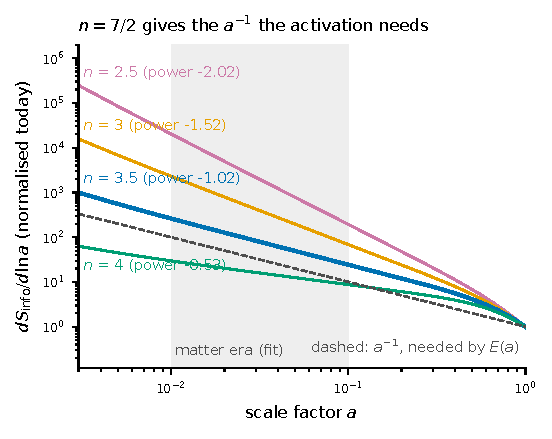
\includegraphics[width=0.62\textwidth]{figures/part2/fig_exponent.pdf}
\caption{$dS_{\rm info}/d\ln a\propto\rho_mD^nf/(T_HA_H)$ with the full $\Lambda$CDM growth factor ($\Omega_m=0.315$, $\Omega_r=9.1\times10^{-5}$), normalised today, for $n=2.5$, 3, 3.5 and 4. The power fitted over the matter era ($0.01\le a\le0.1$, shaded) is $-2.02$, $-1.52$, $-1.02$ and $-0.53$; the activation function needs $a^{-1}$ (dashed), which $n=7/2$ gives. Method of \texttt{docs/verification/scripts/\allowbreak{}verify\_theory\_derivations.py}, section~6. \calc}\label{fig:exponent}
\end{figure}
For the activation function to take the form $\exp(C-1/a)$, we require:
\begin{equation}S_{\rm info}(a)\propto-\frac1a+{\rm const}.\label{eq:th:target}\end{equation}
This requires the integral in Eq.~\eqref{eq:Sn} to yield $a^{-1}$:
\begin{equation}n-\frac92=-1\quad\Longrightarrow\quad n=\frac72 .\label{eq:th:n}\end{equation}
\derived\ The analytically predicted nonlinear exponent is $n=7/2$. It lies between linear ($n=1$) and fully nonlinear ($n\gtrsim4$) structure
formation --- the regime where the majority of information production occurs in the real universe. This value is derived under the matter-domination
approximation. Integrating Eqs.~\eqref{eq:Idot}--\eqref{eq:dSdt} with the full $\Lambda$CDM growth factor gives $dS_{\rm info}/d\ln a\propto a^{-1.02}$ in the
matter era for $n=7/2$ (Fig.~\ref{fig:exponent}) \calc; in the $\Lambda$ era the same $n$ gives a steeper fall ($a^{-1.57}$ over $0.25\le a\le1$), so the full
background raises the effective exponent. Section~\ref{sec:numerics} finds the closest fit to the activation function for $D^{7/2}$. The activation function
itself does not depend on $n$: it follows from the decoherence constraint below.

\subsection{Recovery of the activation function}
With $n=7/2$, the informational entropy is:
\begin{equation}S_{\rm info}(a)\propto-\frac1a+C .\label{eq:th:S72}\end{equation}
The modification to $H^2$ enters through the informational energy density $\rho_{\rm info}$, which is determined by the Cai--Kim first law together
with the standard continuity equation. The informational term in the first law contributes
\begin{equation}-dE_{\rm info}=T_H\,dS_{\rm info}.\label{eq:th:dEinfo}\end{equation}
The decoherence constraint $\dot\varphi=H/a$ (where $\varphi\equiv\ln E(a)=1-1/a$ tracks the cumulative decoherence history) gives
$dS_{\rm info}/dt\propto H/a$, the time derivative of Eq.~\eqref{eq:th:S72}: $d(-1/a)/dt=\dot a/a^2=H/a$. The associated energy density therefore satisfies
\begin{equation}\dot\rho_{\rm info}=\rho_{\rm info}\cdot\frac Ha .\label{eq:th:rhodot}\end{equation}
\conjecture\ (the identification of the energy density's growth rate with the record rate) Equation~\eqref{eq:th:rhodot} is a separable ODE. With
$dt=da/(aH)$, separating variables and integrating directly:
\begin{equation}\rho_{\rm info}(a)\propto\exp\!\Big(\int\frac Ha\,\frac{da}{aH}\Big)=\exp\!\Big(\int\frac{da}{a^2}\Big)=\exp\!\Big(-\frac1a\Big).\label{eq:th:rhoint}\end{equation}
Since $\Delta H^2=(8\pi G/3)\,\rho_{\rm info}$, the modification is:
\begin{equation}\Delta H^2\propto\exp\!\Big(C-\frac1a\Big).\label{eq:th:dH2}\end{equation}
The exponential functional form is therefore not imposed by hand; it follows from integrating the decoherence constraint directly. No assumption about
microstate counting is required. The equation of state $w_{\rm info}=-1-1/(3a)$ is derived independently from the variational formulation in
Section~\ref{sec:var}, confirming this result.

The normalisation constant $C$ is fixed by requiring $E(a{=}1)=1$:
\begin{equation}E(1)=\exp(C-1)=1\quad\Longrightarrow\quad C=1 .\label{eq:th:C}\end{equation}
Therefore:
\begin{equation}\boxed{E(a)=\exp\!\Big(1-\frac1a\Big)}\label{part2:eq:Ea}\end{equation}
\derived\ This is the activation function, now derived from horizon thermodynamics rather than assumed.

\subsection{Physical origin of the $1/a$ term}
The $1/a$ in the exponent has a precise physical meaning. It arises from the ratio of the structure-formation rate to the horizon area:
\begin{equation}\frac{\text{structure formation rate}}{A_H}\propto\frac{D(a)}{A_H(a)}\propto\frac{a}{a^3}=\frac{1}{a^2}.\label{eq:th:surfdens}\end{equation}
Integrating $1/a^2$ yields $-1/a$. \derived\ The activation function is therefore the exponential of the cumulative information surface density on the cosmic
horizon. What drives expansion is not how much total information the universe has produced, but how densely that information is packed on the
horizon surface. \interp

\subsection{Redshift interpretation}
In terms of redshift $z=1/a-1$:
\begin{equation}E(z)=\exp\big(1-(1+z)\big)=\exp(-z)=e\cdot e^{-(1+z)}.\label{eq:th:Ez}\end{equation}
\derived\ The activation function is pure exponential decay with redshift --- the simplest possible functional form for a quantity that grows from zero
at early times to a finite value today. $E(z{=}10)=4.5\times10^{-5}$; $E(z{=}2)=0.135$; $E(z{=}1)=0.368$; $E(z{=}0)=1$; $E\to e=2.718$ as $a\to\infty$. \calc

\subsection{Extension beyond matter domination}
The analytical derivation above assumes pure matter domination. The full cosmological history includes radiation domination at early times and
$\Lambda$ domination at late times. These modify the scaling relations in Eqs.~\eqref{eq:th:Hmd}--\eqref{eq:th:Dmd} and raise the effective nonlinear exponent
in the $\Lambda$ era above the analytical value $n=7/2$. The numerical verification in Section~\ref{sec:numerics} accounts for the full $\Lambda$CDM background
evolution: for $D^{7/2}$ the accumulated record is fitted by $\exp(0.93-1.02/a)$, the coefficient of $1/a$ within $2\,\%$ and the constant within
$7\,\%$ of the analytical prediction. \calc

\subsection{Connection to the perturbation equations via Cai--Kim}
The Cai--Kim formalism provides the theoretical derivation of why the informational entropy term exists and motivates its functional form. When the
total entropy is modified to $S_{\rm total}=S_{\rm geo}+S_{\rm info}$, the first law becomes:
\begin{equation}-dE=T\,dS_{\rm geo}+T\,dS_{\rm info}.\label{eq:th:firstlaw2}\end{equation}
The first term reproduces the standard Friedmann equations exactly as in Cai and Kim. The second term introduces the IAM modification: the
informational entropy production, weighted by the Gibbons--Hawking encoding cost, contributes an additional effective energy density. Its activation
function satisfies $E(a)\to0$ as $a\to0$, $E(1)=1$, and $E(a)\approx0$ at recombination ($E(10^{-3})=e^{-999}$).

Importantly, this term does not modify the background expansion. Applying the informational term at the background level gives
$H_0=61.45$ and $61.52$\,km\,s$^{-1}$\,Mpc$^{-1}$ in the two Level 2b chains, inconsistent with Planck 2018 (Chapters~\ref{ch:dual} and~\ref{ch:level2}) \measured. The physical
mechanism of IAM operates exclusively at the perturbation level: the $\beta_mE(a)$ term enters through the sector split derived in
Section~\ref{sec:th:split}, modifying the effective Hubble friction for matter perturbations while leaving the background Friedmann equation and photon sector
unchanged.

\section{The dual-sector split and the $\mu$--$\Sigma$ mapping}\label{sec:th:split}
\subsection{Modified first law}
\paragraph{Why the informational term vanishes in exact FRW.} An exact Friedmann--Robertson--Walker spacetime is conformally flat, with vanishing
Weyl tensor $C_{\mu\nu\rho\sigma}=0$. Any covariant entropy functional built from inhomogeneous gravitational degrees of freedom --- for example, a
functional depending on $C_{\mu\nu\rho\sigma}C^{\mu\nu\rho\sigma}$ or other curvature deviations from conformal flatness --- therefore vanishes
identically in exact FRW. Since the informational entropy $S_{\rm info}$ is sourced by gravitational decoherence associated with inhomogeneous
structure formation, it must vanish in the homogeneous limit. Consequently, the $\beta_mE(a)$ term cannot appear as a modification of the background
Friedmann equation and instead enters only at the level of matter-sector perturbations.

This is a symmetry argument rather than a proof from first principles: we are requiring that $S_{\rm info}$ be consistent with the symmetries of exact
FRW, not deriving its form from a UV-complete theory of quantum gravity. A complete derivation would require specifying the microscopic coupling between
decoherence events and horizon degrees of freedom, which remains an open problem in quantum gravity. \openprob

With the total horizon entropy $S_{\rm total}=S_{\rm geo}+S_{\rm info}$, the Cai--Kim first law becomes
\begin{equation}-dE=T_H\,d(S_{\rm geo}+S_{\rm info}).\label{eq:th:firstlaw3}\end{equation}
The geometric piece yields the standard Friedmann equation. The informational piece yields an additional contribution:
\begin{equation}H^2=\frac{8\pi G}{3}\rho+\frac\Lambda3+\beta_mE(a)H_0^2 .\label{eq:HIAM}\end{equation}
The additive form of the $\beta_mE(a)H_0^2$ term follows directly from the linearity of the Friedmann equation in energy densities. The informational
energy density derived in Section~\ref{sec:th:activation} is
\begin{equation}\rho_{\rm info}(a)=\frac{3H_0^2}{8\pi G}\,\beta_mE(a),\label{eq:th:rhoinfo}\end{equation}
where the normalisation $E(1)=1$ fixes the amplitude at $a=1$ and $\beta_m$ sets the overall scale, with the virial derivation $\beta_m=\Omega_m/2$
established in Section~\ref{sec:th:coupling}. Substituting into the standard Friedmann equation $H^2=(8\pi G/3)\sum_i\rho_i+\Lambda/3$:
\begin{equation}H^2=\frac{8\pi G}{3}(\rho_m+\rho_{\rm info})+\frac\Lambda3=\frac{8\pi G}{3}\rho_m+\frac\Lambda3+\frac{8\pi G}{3}\cdot\frac{3H_0^2}{8\pi G}\beta_mE(a)
=\frac{8\pi G}{3}\rho_m+\frac\Lambda3+\beta_mE(a)H_0^2 .\label{eq:th:cancel}\end{equation}
\derived\ The $8\pi G/3$ factors cancel exactly, leaving $\beta_mE(a)H_0^2$ as a dimensionally consistent additive term. This is not a new assumption;
it is the standard consequence of treating $\rho_{\rm info}$ as a gravitating energy density alongside matter and radiation.

Equation~\eqref{eq:HIAM} represents the formal output of the Cai--Kim first law when $S_{\rm info}>0$. It is an intermediate result in the derivation,
not a claim about the background expansion; the resolution --- why $\beta_mE(a)$ does not modify the background --- follows from the causal structure of
decoherence derived below. The $\beta_mE(a)$ term does not modify the global background: IAM operates at the perturbation level, entering through the
effective Hubble friction $2H_{\rm IAM}\dot\delta_m$ in the matter growth equation, where $H_{\rm IAM}$ (the matter-sector rate, $H_m$ in
Chapter~\ref{ch:dual}) is the rate of Eq.~\eqref{eq:HIAM}. The standard $\Lambda$CDM Friedmann equation correctly describes the background, as confirmed by the
sector split below.

\subsection{The causal origin of the sector split}
The preceding argument applies to degrees of freedom that undergo gravitational decoherence. The causal structure of spacetime determines which
degrees of freedom are affected.

\begin{quote}
\textbf{Definition (decoherence eligibility).} A degree of freedom undergoes gravitational decoherence if and only if it propagates on a timelike
worldline ($d\tau>0$). \conjecture
\end{quote}
The physical basis is that decoherence is a dynamical process requiring a finite proper-time interval $\Delta\tau>0$ for the system--environment
interaction in Eq.~\eqref{eq:th:entangle} to produce orthogonalisation of environmental states. The decoherence timescale $\tau_D$ is finite and positive. For a
degree of freedom with proper-time interval $\Delta\tau$, decoherence occurs when $\Delta\tau\gg\tau_D$.

Massive particles (baryons, dark matter) propagate on timelike worldlines: $\Delta\tau>0$. They interact gravitationally, cluster, virialise, and
decohere. They produce informational entropy.

Photons propagate on null worldlines: $ds^2=0$, $\Delta\tau=0$. A photon does not experience proper time. It does not undergo a temporal sequence of
gravitational interactions. It does not decohere through gravitational clustering. It produces no informational entropy through this channel.

\begin{quote}
\textbf{Proposition (dual-sector coupling).} Let $S_{\rm info}$ denote the informational entropy from gravitational decoherence. Then:
(1) for matter (timelike worldlines), $S_{\rm info}>0$, and the modified first law yields $\mu(a)<1$;
(2) for photons (null worldlines), $S_{\rm info}=0$, and the standard first law yields $\Sigma(a)=1$. \derived\ (given the definition)
\end{quote}
When $S_{\rm info}=0$, the first law reduces to $-dE=T_H\,dS_{\rm geo}$, which yields standard GR. When $S_{\rm info}>0$, the additional entropy modifies
the gravitational coupling for the matter sector.

An important clarification: the sector split does not mean that gravity literally treats null and timelike degrees of freedom differently at the
level of the field equations. The Einstein equations remain universal. Rather, the informational entropy $S_{\rm info}$ --- which enters through the
horizon first law --- is produced exclusively by timelike degrees of freedom. The result is an emergent, sector-dependent renormalisation of the
effective gravitational coupling: matter experiences a weaker effective $G$ because part of the gravitational energy budget is diverted to
informational entropy production, while photons, which do not participate in this process, experience the standard coupling. Diffeomorphism
invariance is preserved because the modification enters through the entropy functional, not through the metric or connection. \interp

\subsection{Mapping to $\mu$--$\Sigma$}
The $\mu$--$\Sigma$ parameterisation~\cite{PogosianSilvestri2016} encodes deviations from GR through:
\begin{gather}
k^2\Phi=-4\pi G\,\mu(a)\,a^2\bar\rho_m\delta_m,\label{eq:th:mudef}\\
k^2(\Phi+\Psi)=-8\pi G\,\Sigma(a)\,a^2\bar\rho_m\delta_m.\label{eq:th:sigmadef}
\end{gather}
The proposition maps onto this framework.
\emph{Matter sector ($\mu$).} The informational entropy modifies the coupling governing density perturbations:
\begin{equation}\mu(a)=\frac{H^2_{\Lambda\rm CDM}(a)}{H^2_{\Lambda\rm CDM}(a)+\beta_mE(a)H_0^2}.\label{eq:th:mu}\end{equation}
At $a=1$, where $H_{\Lambda\rm CDM}=H_0$ and $E=1$:
\begin{equation}\mu_0\equiv\mu(z{=}0)-1=\frac{-\beta_m}{1+\beta_m}=-0.136 .\label{eq:th:mu0}\end{equation}
\derived\ ($\mu(0)=1/(1+\beta_m)=0.8638$, $\mu_0=-0.1362$ \calc) \emph{Photon sector ($\Sigma$).} Since $S_{\rm info}=0$ for null degrees of freedom:
\begin{equation}\Sigma(a)=1\quad\text{(exact)}.\label{eq:th:Sigma}\end{equation}
\derived\ This is the central prediction: $\mu<1$, $\Sigma=1$. \prediction\ The suppression $\mu<1$ means that matter perturbations grow more slowly than in GR.
The preservation $\Sigma=1$ means that CMB anisotropies, gravitational lensing, and BAO angular positions are unaffected.

\begin{figure}[htbp]\centering
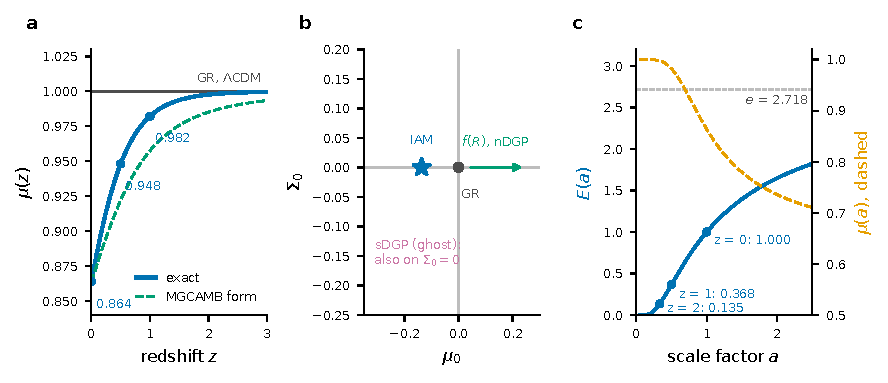
\includegraphics[width=\textwidth]{figures/part2/fig_theory_mu_sigma.pdf}
\caption{The prediction in the $\mu$--$\Sigma$ framework. (a) The gravitational coupling $\mu(z)=H^2/(H^2+\beta_mE(a)H_0^2)$ (solid), with the
$\Lambda$CDM baseline $\mu=1$ and the MGCAMB parameterisation $\mu=1+\mu_0\,\Omega_{\rm DE}(a)/\Omega_{\rm DE}$ (dashed), which equals the exact form at
$z=0$ and departs from it by at most $2.8\,\%$, near $z\approx0.64$. Values at key redshifts: $\mu(0)=0.864$, $\mu(0.5)=0.948$, $\mu(1)=0.982$.
(b) The $(\mu_0,\Sigma_0)$ plane in the quasi-static regime: the IAM point $(-0.136,0)$; $f(R)$ gravity and the normal branch of DGP move along
$\Sigma_0=0$ toward $\mu_0>0$; the self-accelerating DGP branch also gives $\mu_0<0$, $\Sigma_0=0$ but carries a ghost. (c) The activation function
$E(a)=\exp(1-1/a)$ (solid, left axis) grows from zero at early times toward saturation at $e\approx2.718$; the coupling $\mu(a)$ (dashed, right axis)
shows the suppression increasing toward the present epoch. $\Omega_m=0.3153$, $\beta_m=\Omega_m/2$. Script \texttt{docs/book/figscripts/\allowbreak{}fig\_p2\_theory\_derivations.py}. \calc}\label{fig:th:musigma}
\end{figure}

\section{Variational formulation}\label{sec:var}
We now show that the thermodynamic result admits a variational formulation, establishing the connection to standard field-theoretic language.

\begin{figure}[htbp]\centering
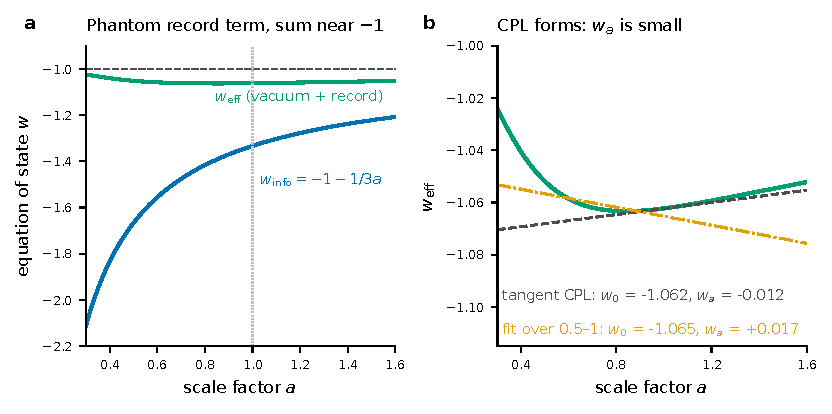
\includegraphics[width=\textwidth]{figures/part2/fig_w_eff.pdf}
\caption{(a) The record term's equation of state $w_{\rm info}=-1-1/(3a)$ and the combined dark sector $w_{\rm eff}=[-\Omega_\Lambda+\beta E(a)w_{\rm info}]/[\Omega_\Lambda+\beta E(a)]$ ($\Omega_m=0.315$). (b) $w_{\rm eff}$ and its two CPL forms: the tangent at $a=1$ ($w_0=-1.062$, $w_a=-\Omega_m^2/3(2-\Omega_m)^2=-0.012$) and a least-squares fit over $0.5\le a\le1$ ($w_0=-1.065$, $w_a=+0.017$). \derived\ (form) \calc\ (values)}\label{fig:w_eff}
\end{figure}

\subsection{The informational scalar field}
Define the scalar field
\begin{equation}\varphi(t)\equiv\ln E(a)=1-\frac1a .\label{eq:th:phi}\end{equation}
This field satisfies
\begin{equation}\dot\varphi=\frac{\dot a}{a^2}=\frac Ha .\label{eq:th:phidot}\end{equation}
\derived\ Equation~\eqref{eq:th:phidot} is a constraint, not a Klein--Gordon equation. The field $\varphi$ does not propagate independently; its evolution
is determined by the background geometry. Physically, $\varphi$ tracks the cumulative decoherence history: it is a thermodynamic variable, not a
dynamical degree of freedom.

\subsection{The constrained action}
The total gravitational action is
\begin{equation}S=S_{\rm EH}+S_\Lambda+S_{\rm matter}+S_{\rm info},\label{eq:th:Stot}\end{equation}
where $S_{\rm EH}$ is the Einstein--Hilbert action, $S_\Lambda$ is the cosmological-constant term, $S_{\rm matter}$ is the matter action, and
\begin{equation}S_{\rm info}=\int\Big[-\frac{3H_0^2}{8\pi G}\beta_m e^{\varphi}+\lambda\Big(\dot\varphi-\frac Ha\Big)\Big]\sqrt{-g}\,d^4x .\label{eq:th:action}\end{equation}
\conjecture\ (the action) The first term is the informational energy density $\rho_{\rm info}=(3H_0^2/8\pi G)\beta_me^{\varphi}$. The second term, with
Lagrange multiplier $\lambda$, enforces the decoherence constraint~\eqref{eq:th:phidot}.

\subsection{Variation}
Restricted to FRW symmetry, $ds^2=-N^2dt^2+a^2d\mathbf x^2$, so $\sqrt{-g}=Na^3$, and the proper-time derivatives are $\dot\varphi=\varphi'/N$ and
$H=a'/(aN)$ (prime $=d/dt$). The Lagrangian of Eq.~\eqref{eq:th:action} per unit comoving volume is then
\begin{equation}L_{\rm info}=-Na^3\rho_{\rm info}(\varphi)+\lambda\,a^3\Big(\varphi'-\frac{a'}{a^2}\Big):\label{eq:th:Lmini}\end{equation}
the constraint term carries no lapse. Three independent variations yield three results.

\emph{Variation with respect to $\lambda$.} Produces the constraint $\dot\varphi=H/a$, which determines the field evolution.

\emph{Variation with respect to $\varphi$.} The Euler--Lagrange equation $\partial L/\partial\varphi-d(\partial L/\partial\varphi')/dt=0$ gives
\begin{equation}\frac{d}{dt}\big(a^3\lambda\big)=-a^3\rho_{\rm info}\qquad\Longleftrightarrow\qquad\dot\lambda+3H\lambda=-\frac{3H_0^2}{8\pi G}\beta_me^{\varphi},\label{eq:th:lambdadot}\end{equation}
which determines the Lagrange multiplier. \derived\ This is an auxiliary equation with no independent physical content: $\lambda$ enforces the
thermodynamic constraint and is not independently observable.

\emph{Variation with respect to $g_{ab}$.} Produces the modified Einstein equation. Restricted to FRW symmetry, the variation with respect to the lapse
(the Hamiltonian constraint) receives $-a^3\rho_{\rm info}$ from Eq.~\eqref{eq:th:Lmini} and nothing from the constraint term, and so yields the modified
Friedmann equation~\eqref{eq:HIAM}:
\begin{equation}H^2=\frac{8\pi G}{3}(\rho_m+\rho_r)+\frac\Lambda3+\beta_me^{\varphi}H_0^2 .\label{eq:th:Hvar}\end{equation}
\derived\ With the constraint $\varphi=1-1/a$, this is identically Eq.~\eqref{eq:HIAM}. The action principle reproduces the thermodynamic result exactly. As
written, the action places the term in the Friedmann equation for every component; that it acts on the matter sector only is the sector rule of
Section~\ref{sec:th:split}, applied separately.

\subsection{Equation of state}
The informational energy density $\rho_{\rm info}=(3H_0^2/8\pi G)\beta_mE(a)$ evolves as
\begin{equation}\dot\rho_{\rm info}=\rho_{\rm info}\cdot\frac Ha .\label{eq:th:rhodot2}\end{equation}
Substituting into the continuity equation $\dot\rho+3H(\rho+P)=0$, $\dot\rho_{\rm info}/\rho_{\rm info}=-3H(1+w_{\rm info})=H/a$:
\begin{equation}w_{\rm info}(a)=-1-\frac{1}{3a}.\label{eq:th:winfo}\end{equation}
\derived\ This is a mildly phantom equation of state ($w<-1$) at all finite $a$, approaching $w\to-1$ as $a\to\infty$. At the present epoch,
$w_{\rm info}(1)=-4/3$.

The phantom behaviour has a transparent origin: the informational energy density grows faster than volumetric dilution because structure formation
continuously produces new information. The factor $1/3$ arises from the three spatial dimensions; the factor $1/a$ from the information production
rate. The equation of state is determined entirely by geometry and information.

This does not violate the null energy condition, because $\varphi$ is a thermodynamic variable constrained by the geometry, not a propagating field
with kinetic energy.

\subsection{Combined dark-energy equation of state}
The total dark-energy sector includes both the cosmological constant and the informational contribution. The effective equation of state for the
combined sector is:
\begin{equation}w^{\rm eff}_{\rm DE}(a)=\frac{P_\Lambda+P_{\rm info}}{\rho_\Lambda+\rho_{\rm info}}=\frac{-\rho_\Lambda+w_{\rm info}\,\rho_{\rm info}}{\rho_\Lambda+\rho_{\rm info}}.\label{eq:th:weff}\end{equation}
With $\rho_\Lambda=\Omega_\Lambda\cdot3H_0^2/(8\pi G)$ and $\rho_{\rm info}=\beta_mE(a)\cdot3H_0^2/(8\pi G)$, and $\Omega_\Lambda=1-\Omega_m$,
$\beta_m=\Omega_m/2$, the value at $a=1$ is
\begin{equation}w^{\rm eff}_{\rm DE}(1)=\frac{-\Omega_\Lambda-\tfrac43\beta_m}{\Omega_\Lambda+\beta_m}=-\frac{1-\Omega_m/3}{1-\Omega_m/2}=-1.062 .\end{equation}
In the CPL parameterisation~\cite{ChevallierPolarski2001,Linder2003} $w(a)=w_0+w_a(1-a)$, the IAM prediction is obtained by matching $w^{\rm eff}(a)$ and its
derivative $dw/da$ to the CPL form at $a=1$. With $E(1)=E'(1)=1$, $w_{\rm info}(1)=-4/3$ and $w'_{\rm info}(1)=1/3$, differentiating
Eq.~\eqref{eq:th:weff} gives $dw^{\rm eff}/da|_{1}=\beta_m^2/[3(\Omega_\Lambda+\beta_m)^2]$, so
\begin{equation}w_0=-1.062,\qquad w_a=-\frac{dw^{\rm eff}}{da}\Big|_{a=1}=-\frac{\Omega_m^2}{3(2-\Omega_m)^2}=-0.012 .\end{equation}
\derived\ (form) \calc\ ($\Omega_m=0.315$) $w_a$ is small and of fixed sign for $\Omega_m=0.30$--$0.32$; a least-squares CPL fit over $0.5\le a\le1$ gives
$w_0=-1.065$, $w_a=+0.017$ (Fig.~\ref{fig:w_eff}). Either way the model's dark-energy sector stays close to $w_a=0$ and below $w=-1$, a mild phantom
departure from $\Lambda$CDM; what distinguishes it is the split between distance and growth probes (Section~\ref{sec:th:predictions}, item~1), not a large $w_a$.

\subsection{Nature of the informational field}
The constrained scalar field $\varphi$ is fundamentally different from standard quintessence or phantom dark-energy fields. It has no independent
dynamics --- its evolution is fixed by the constraint $\dot\varphi=H/a$, not by a Klein--Gordon equation. It has no kinetic energy in the usual sense ---
the ``velocity'' $\dot\varphi$ is a geometric quantity, not a canonical momentum. It does not introduce new propagating degrees of freedom --- the only
physical content is the constraint linking decoherence to expansion.

The field $\varphi$ is not a new particle or a dark-energy component in the conventional sense. It is a thermodynamic variable --- an entropy --- that
tracks cumulative decoherence, analogous to the way temperature is determined by the state of a gas rather than by its own equation of motion. The
Lagrange-multiplier formulation is the natural variational language for such constrained thermodynamic systems. \interp

\section{The coupling constant: $\beta_m=\Omega_m/2$}\label{sec:th:coupling}
\subsection{The virial partition}
The virial theorem for gravitationally bound systems states that the time-averaged kinetic energy equals minus half the time-averaged potential
energy:
\begin{equation}\langle T\rangle=-\frac12\langle V\rangle .\label{eq:th:virialavg}\end{equation}
In the IAM framework, gravitational collapse produces two effects: (i) it curves spacetime, contributing to the geometric entropy $S_{\rm geo}$ (this is
standard general relativity), and (ii) it decoheres quantum superpositions into classical information, contributing to the informational entropy
$S_{\rm info}$. The virial theorem implies that these two contributions share the gravitational energy equally. \conjecture\ (the equal share) The
informational energy density at the present epoch is therefore:
\begin{equation}\rho_{\rm info}(a{=}1)=\frac12\rho_m=\frac{\Omega_m}{2}\rho_{\rm crit}.\label{eq:th:rhoinfo1}\end{equation}
Since $\rho_{\rm info}(a{=}1)=\beta_mE(1)\rho_{\rm crit}=\beta_m\rho_{\rm crit}$, this gives:
\begin{equation}\beta_m=\frac{\Omega_m}{2}.\label{eq:th:betam}\end{equation}
\derived\ With $\Omega_m=0.3153$ (Planck 2018~\cite{Planck2018VI}), the prediction is $\beta_m=0.15765$ \calc. It is held fixed, not fitted, in every chain of
Chapters~\ref{ch:dual} and~\ref{ch:level2}.

\subsection{Comparison with published mass functions}
Integration of N-body-calibrated halo mass functions shows what the factor $\tfrac12$ is not. Using the Sheth--Tormen~\cite{ShethTormen1999} and Tinker et
al.~\cite{Tinker2008} mass functions with Planck 2018 cosmological parameters ($h=0.674$, $\Omega_bh^2=0.0224$, $\sigma_8=0.811$, $n_s=0.965$) and the
Eisenstein--Hu transfer function~\cite{EisensteinHu1998} (no-wiggle form), the collapsed fraction of matter in halos with $M>10^6\,M_\odot$ at $z=0$ is:
\begin{equation}f^{\rm ST}_{\rm coll}=0.64,\qquad f^{\rm Tinker}_{\rm coll}=0.71 .\label{eq:th:fcoll}\end{equation}
\calc\ The mass threshold extrapolates the Tinker fit below its calibrated range ($\gtrsim10^{10.5}M_\odot$), and $f_{\rm coll}$ depends on it.
The naive prediction $\beta_m=\Omega_m\,f_{\rm coll}=0.20$--$0.22$ lies $27$--$41\,\%$ above $\Omega_m/2$. The collapsed fraction is therefore not the
primary explanation of the coupling; the factor $\tfrac12$ comes from the equipartition of gravitational energy, not from counting halos. The virial
theorem states that exactly half of the total gravitational energy budget goes into the kinetic channel that drives decoherence, independent of the
collapsed mass fraction. Writing the coupling as
\begin{equation}\beta_m=\Omega_m\cdot f_{\rm coll}\cdot\eta_{\rm vir}\label{eq:th:betadecomp}\end{equation}
defines the virial efficiency $\eta_{\rm vir}\equiv1/(2f_{\rm coll})\approx0.7$--$0.8$; with this definition Eq.~\eqref{eq:th:betadecomp} equals
$\Omega_m/2$ identically, so it is a rewriting, not a test. \derived\ The virial theorem captures both factors in one step:
$\langle T\rangle=-\tfrac12\langle V\rangle\Rightarrow\beta_m=\Omega_m/2$.

Published simulations measure the halo virial ratio $2T/|U|$ within $r_{\rm vir}$ at or slightly above unity: Neto et al.\ (2007)~\cite{Neto2007}
find the median ``slightly greater than unity'' and select relaxed halos by $2T/|U|<1.35$; Power, Knebe and Knollmann (2012~\cite{Power2012}, Eqs.~17--18) find
$\eta=2T/|W|\approx1.15$ at $10^{12}\,h^{-1}M_\odot$ rising to $\approx1.25$ at $10^{15}\,h^{-1}M_\odot$, the excess coming from halos still accreting.
\observed\ $\eta_{\rm vir}$ above is therefore a definition, $1/(2f_{\rm coll})$, not a simulation measurement, and $\beta_m=\Omega_m/2$ rests on the
virial partition itself.

\subsection{Testable prediction}
The relation $\beta_m=\Omega_m/2$ is a specific, falsifiable prediction: the ratio $\beta_m/\Omega_m=1/2$ should hold for any value of $\Omega_m$. Since
$\beta_m$ is fixed rather than fitted in the chains, the test with existing data is the analysis with $\mu_0$ left free (Chapter~\ref{ch:dual}), and future growth
data will sharpen it. \prediction

\subsection{Parameter count}
With $\beta_m=\Omega_m/2$, the IAM model has zero free parameters beyond those already present in $\Lambda$CDM:
\begin{itemize}
\item The activation function $E(a)=\exp(1-1/a)$: derived from horizon thermodynamics (Section~\ref{sec:th:activation}).
\item The $1/a$ coefficient: derived from information surface density (Eq.~\eqref{eq:th:surfdens}) and the exponent $n=7/2$; the full-background integration of
Section~\ref{sec:numerics} gives $1.02$ for $D^{7/2}$.
\item The normalisation $E(1)=1$: set by definition.
\item The coupling constant $\beta_m=\Omega_m/2$: derived from the virial theorem.
\end{itemize}
The entire modification to $\Lambda$CDM --- the functional form, the exponent, the normalisation, and the amplitude --- is determined by established
physics, the one identification of Section~\ref{sec:th:info}, and the independently measured matter density $\Omega_m$. IAM is a zero-parameter extension of
$\Lambda$CDM.

\subsection{Independence from microscopic details}
A natural question is whether the derivation requires knowledge of the microscopic information production rate --- specifically, how many bits of
classical information a single collapsing halo produces. It does not.

The functional form $E(a)=\exp(1-1/a)$ depends on the scaling of the decoherence rate with scale factor, not on its absolute normalisation. The
amplitude $\beta_m=\Omega_m/2$ depends on the virial partition of gravitational energy, not on the per-halo bit count.

This is standard thermodynamic reasoning: macroscopic behaviour is determined by scaling laws and conservation principles, not by the enumeration of
microstates. Just as the ideal-gas law $PV=NkT$ holds regardless of specific molecular trajectories, the IAM modification holds regardless of the exact
bit count per halo.

\section{Numerical verification}\label{sec:numerics}
To verify the analytical derivation, we numerically compute the cumulative decoherence integral using the full $\Lambda$CDM background cosmology
($\Omega_m=0.315$, $\Omega_r=9.1\times10^{-5}$, $H_0=67.4$\,km\,s$^{-1}$\,Mpc$^{-1}$).

\subsection{Source-term models}
We test multiple physically motivated source terms for the decoherence rate, ranging from simple power laws ($D^n$) to Press--Schechter and
Sheth--Tormen models with exponential sensitivity to the growth factor. Each is combined with the Gibbons--Hawking encoding factor of
Eq.~\eqref{eq:dSdt} ($1/(T_HA_H)=H/2$) and integrated cumulatively per unit time:
\begin{equation}I(a)=\int_0^{t(a)}\frac{R(a')}{T_H(a')\,A_H(a')}\,dt'=\int_0^a\frac{R(a')}{T_H(a')\,A_H(a')}\,\frac{da'}{a'H(a')}\;\propto\;\int_0^a\frac{R(a')}{a'}\,da',\label{eq:th:Iint}\end{equation}
where $R(a)$ is the instantaneous decoherence rate per Hubble time: $R=\Omega_m(a)\,f\,D^n$ for the power laws and $R=\Omega_m(a)\,dF/d\ln a$ for a
collapsed fraction $F$. (With the full rate $\rho_mD^nfH$ of Eq.~\eqref{eq:Idot} the integral from $a=0$ diverges for every $n\le9/2$, since the integrand goes as
$a^{n-11/2}$; for that rate only the slope test of Fig.~\ref{fig:exponent} is defined.)

\subsection{Results}
Table~\ref{tab:th:record} summarises the results. The cumulative integral is normalised to unity at $a=1$ and fitted to the functional form
$\exp(\alpha-\beta/a)$ over $0.15\le a\le2.0$. The target is $\alpha=\beta=1$.

\begin{table}[htbp]\centering\small
\caption{Numerical verification: fitted coefficients $\alpha$ and $\beta$ for the cumulative decoherence integral $I(a)\propto\exp(\alpha-\beta/a)$,
Eq.~\eqref{eq:th:Iint}, compared with the target $\alpha=\beta=1$. The Pearson correlation $r$ is computed over $0.15\le a\le2.0$. The first row omits the
horizon factor $1/(T_HA_H)$. Collapsed fractions: $F_{\rm PS}=\mathrm{erfc}(\nu/\sqrt2)$ and the Sheth--Tormen $F_{\rm ST}(\nu)=\int_\nu^\infty f_{\rm ST}(\nu')\,d\nu'/\nu'$,
$\nu=\delta_c/(\sigma_*D)$. \calc}\label{tab:th:record}
\begin{tabular}{lccc}\toprule
Source model $R$ & $\alpha$ & $\beta$ & $r$\\\midrule
$D^2\,\Omega_m(a)\,f$ (no horizon factor) & 0.85 & 0.96 & 0.993\\
$D^2\,\Omega_m(a)\,f$ & 0.53 & 0.59 & 0.995\\
$D^{5/2}\,\Omega_m(a)\,f$ & 0.66 & 0.74 & 0.995\\
$D^{3}\,\Omega_m(a)\,f$ & 0.79 & 0.88 & 0.994\\
$D^{7/2}\,\Omega_m(a)\,f$ & 0.93 & 1.02 & 0.994\\
$D^{4}\,\Omega_m(a)\,f$ & 1.06 & 1.16 & 0.994\\
Press--Schechter, $\sigma_*=1.0$ & 1.06 & 1.24 & 0.983\\
Press--Schechter, $\sigma_*=1.2$ & 0.86 & 1.02 & 0.982\\
Sheth--Tormen, $\sigma_*=1.0$ & 0.90 & 1.07 & 0.983\\
Sheth--Tormen, $\sigma_*=1.2$ & 0.75 & 0.89 & 0.982\\
Target: $E(a)$ & 1.00 & 1.00 & 1.000\\\bottomrule
\end{tabular}
\end{table}

\begin{figure}[htbp]\centering
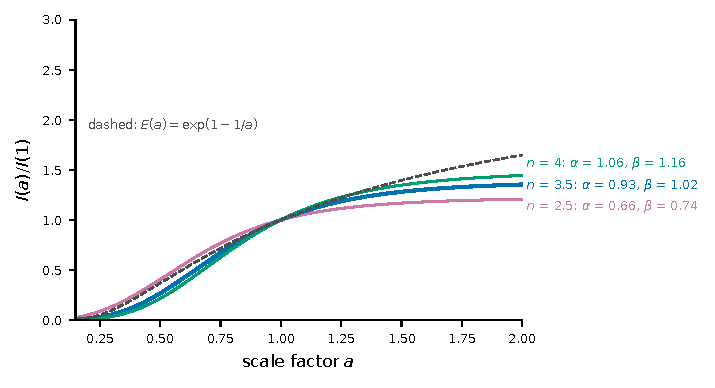
\includegraphics[width=0.62\textwidth]{figures/part2/fig_record_fit.pdf}
\caption{The accumulated record $I(a)/I(1)$ of Eq.~\eqref{eq:th:Iint} for $R=\Omega_m(a)fD^n$, $n=2.5$, $3.5$ and $4$, against the activation function
$E(a)=\exp(1-1/a)$ (dashed), with the coefficients of the fit $\exp(\alpha-\beta/a)$ over $0.15\le a\le2$. Full $\Lambda$CDM background. Script
\texttt{docs/book/figscripts/\allowbreak{}fig\_p2\_theory\_derivations.py}. \calc}\label{fig:th:recordfit}
\end{figure}
The best agreement among the power laws is obtained for $D^{7/2}$ with the Gibbons--Hawking factor, yielding $\exp(0.93-1.02/a)$ --- the coefficient of
$1/a$ within $2\,\%$ and the constant within $7\,\%$ of the target. The analytical prediction $n=7/2$ is thus also the power law closest to the
activation function over the full history (Fig.~\ref{fig:th:recordfit}). \calc

The effective exponent $n\approx3.5$ is physically reasonable: it lies between the linear regime ($n=1$) relevant at early times and the fully
nonlinear regime ($n\ge4$) relevant for collapsed halos, representing the transition region where the majority of cosmic information production occurs.
\interp

\subsection{Coefficient convergence}
Both $\alpha$ and $\beta$ increase monotonically with $n$ and cross through unity in the range $n\approx3$--$4$. The $\alpha=1$ crossing occurs near
$n\approx3.8$, while $\beta=1$ crosses near $n\approx3.4$ \calc. The fact that both crossings occur in the same range, around the analytical $n=7/2$,
supports the interpretation that the activation function is not accidental. The fits test the shape of the accumulated record; its amplitude is set
separately, by $\beta_m$.

\subsection{Sheth--Tormen halo mass function}
To move beyond power-law approximations, we replace $D^n$ with the Sheth--Tormen (ST) multiplicity function~\cite{ShethTormen1999}, which gives the rate at which
mass collapses into halos as a function of the peak height $\nu=\delta_c/(\sigma_*D(a))$, where $\sigma_*$ is the RMS density fluctuation at a
characteristic mass scale:
\begin{equation}f_{\rm ST}(\nu)=A\sqrt{\frac{2q}{\pi}}\Big[1+(q\nu^2)^{-p}\Big]\,\nu\,e^{-q\nu^2/2},\label{eq:th:fST}\end{equation}
with $A=0.3222$, $q=0.707$, $p=0.3$. The cumulative decoherence integral using the ST collapse rate with the Gibbons--Hawking factor
(Eq.~\eqref{eq:th:Iint}) is computed for a range of characteristic $\sigma_*$ values (Table~\ref{tab:th:record}). The coefficient of $1/a$ passes through unity for
$\sigma_*$ between 1.0 and 1.2 (ST: $\beta=1.07$ at $\sigma_*=1.0$, $0.89$ at $1.2$), the range of galaxy-scale halos where the bulk of cosmic structure
formation occurs, and the Press--Schechter collapse rate gives $\beta=1.02$ at $\sigma_*=1.2$. \calc\ The galaxy-scale collapse rate, weighted by
horizon thermodynamics, thus produces a $1/a$ dependence with a coefficient near unity, consistent with the interpretation that the $1/a$ has a
physical origin in the halo collapse rate weighted by horizon thermodynamics.

We note that the Sheth--Tormen mass function is calibrated against $\Lambda$CDM N-body simulations, so this result is not fully independent of the
assumed background cosmology. However, the virial-theorem derivation of $\beta_m=\Omega_m/2$ (Section~\ref{sec:th:coupling}) is independent of any mass-function
calibration and provides the primary determination of the coupling constant. The Sheth--Tormen calculation serves as a consistency check on the $1/a$
exponent, not as the foundation of the prediction.

Every step of this derivation chain --- from the Jacobson thermodynamic identity through the accumulated integral --- is reproduced, symbolically
where algebraic and numerically where a number appears, by \texttt{docs/verification/scripts/\allowbreak{}verify\_theory\_derivations.py} (output beside it).

\section{Perturbation theory: $\mu(a)<1$, $\Sigma(a)=1$}\label{sec:th:pert}
\subsection{The informational field does not fluctuate}
\paragraph{Perturbative status of $\delta\varphi$.} The scalar $\varphi$ is defined through the background apparent-horizon radius $\tilde r_A=1/H(t)$
and therefore depends only on the homogeneous expansion rate. In linear scalar perturbation theory, perturbations are evaluated at fixed background
$H(t)$, while local overdensities source metric potentials $\Psi$ and $\Phi$ without shifting the background-defined apparent horizon at first order.
Under this standard separation between background and perturbations, $\delta\varphi$ vanishes to first order. Higher-order backreaction effects are
beyond the scope of the present analysis.

The constrained scalar field $\varphi=1-1/a$ is defined by the Cai--Kim first law~\cite{CaiKim2005} applied to the cosmic apparent horizon. The apparent horizon is a
global (background) surface determined by the volume-averaged expansion rate $H(t)$, not by local density perturbations. Local overdensities $\delta\rho$
produce gravitational potentials $\Psi$ and $\Phi$, but they do not change the apparent-horizon radius $\tilde r_A=1/H$ at first order in perturbation
theory. Therefore
\begin{equation}\delta\varphi=0\label{eq:th:dphi}\end{equation}
in linear perturbation theory. \derived\ This is analogous to the cosmological constant, which satisfies $\delta\Lambda=0$: both are properties of the
spacetime geometry, not of the local matter content.

Formally, perturbing the constrained action Eq.~\eqref{eq:th:action}: variation with respect to $\lambda$ gives the perturbed constraint $\delta\dot\varphi=0$
(since the horizon expansion rate is unperturbed at first order), and combined with the initial condition $\delta\varphi=0$, the field remains
unperturbed at all times.

\subsection{Standard GR perturbations with the matter-sector expansion rate}
With $\delta\varphi=0$, the cosmological perturbation equations are identical to standard general relativity, evaluated with the matter-sector
expansion rate. In the conformal Newtonian gauge ($ds^2=a^2[-(1+2\Psi)\,d\tau^2+(1-2\Phi)\,d\mathbf x^2]$):
the Poisson equation
\begin{equation}k^2\Psi=-4\pi Ga^2\rho_m\delta_m ;\label{eq:th:poisson}\end{equation}
the anisotropic-stress relation
\begin{equation}\Psi=\Phi\label{eq:th:noaniso}\end{equation}
(no anisotropic stress from the informational sector, since $\delta\varphi=0$); and the growth equation
\begin{equation}\ddot\delta_m+2H_{\rm IAM}\dot\delta_m-4\pi G\rho_m\delta_m=0 .\label{eq:th:growth}\end{equation}
\derived\ These are exactly the standard GR equations. The only difference from $\Lambda$CDM is that matter perturbations feel the matter-sector rate
$H_{\rm IAM}$ of Eq.~\eqref{eq:HIAM}, larger than $H_{\Lambda\rm CDM}$ by the $\beta_mE(a)$ term, as friction; the background expansion is unchanged. The
enhanced Hubble friction $2H_{\rm IAM}\dot\delta_m$ suppresses growth relative to $\Lambda$CDM. At fixed cosmological parameters and the same early
amplitude, the growth factor today is lower by $0.67\,\%$ with Eq.~\eqref{eq:th:growth} (background clock unchanged) and by $0.78\,\%$ with $G_{\rm eff}=\mu G$
on the $\Lambda$CDM background \calc.

Numerical validation via modified CAMB~\cite{Lewis2000CAMB} (Level 2, three converged chains against the full Planck 2018 likelihood) confirms that the
modified expansion rate $H_{\rm IAM}$ operates within the matter-sector perturbation equations (as \texttt{adotoa\_matter} in the Boltzmann solver),
while the global background Friedmann equation remains standard $\Lambda$CDM. Two exploratory runs with the modification applied at the background
level (Level 2b) produced $H_0\approx61.5$\,km\,s$^{-1}$\,Mpc$^{-1}$, confirming that the standard $\Lambda$CDM background is correct and the dual-sector split
is a perturbation-level effect. The Level 2 validation yields $\Delta\chi^2=+0.54$ (best fit) relative to $\Lambda$CDM under the full Planck likelihood,
with $\sigma_8$ shifting from $0.809$ to $0.800$ and $H_0({\rm matter})=72.26$\,km\,s$^{-1}$\,Mpc$^{-1}$, $0.75\sigma$ from SH0ES (Chapter~\ref{ch:level2}). \measured

\subsection{Derived $\mu(a)$ and $\Sigma(a)$}
Since the IAM perturbation equations are standard GR (no modifications to the Poisson equation, no anisotropic stress), the $\mu$--$\Sigma$ values when
mapped relative to the $\Lambda$CDM background are:
\begin{equation}\mu(a)=\frac{E^2_{\Lambda\rm CDM}(a)}{E^2_{\rm IAM}(a)}<1,\qquad\Sigma(a)=1,\label{eq:th:mu2}\end{equation}
with $E^2_{\Lambda\rm CDM}=H^2_{\Lambda\rm CDM}/H_0^2$ and $E^2_{\rm IAM}=E^2_{\Lambda\rm CDM}+\beta_mE(a)$, the same as Eq.~\eqref{eq:th:mu}. \derived\ The effective $\mu<1$
arises because the enhanced Hubble friction lowers the effective matter density parameter seen by perturbations, $4\pi G\rho_m/H^2_{\rm IAM}$, below its
$\Lambda$CDM value, so matter clusters less effectively. Numerically: $\mu(z{=}0)=0.864$, $\mu(z{=}0.5)=0.948$, $\mu(z{=}1)=0.982$, with $\mu\to1$ at
high redshift as $E(a)\to0$ ($\mu(z{=}3)=0.9996$) \calc.

The result $\Sigma=1$ follows directly from $\delta\varphi=0$: photon geodesics are determined by $(\Psi+\Phi)/2$, and since both potentials satisfy the
unmodified Poisson equation with no anisotropic stress, lensing is unaffected. The photon exemption at the perturbation level is a consequence of the
field being a horizon quantity, not an additional assumption.

\subsection{Distinction from other modified gravity theories}
The prediction $\mu<1$, $\Sigma=1$ occupies a distinctive region of the $\mu$--$\Sigma$ parameter space (Fig.~\ref{fig:th:musigma}b). Most extensions of
gravity strengthen growth: $f(R)$~\cite{PogosianSilvestri2008} and the normal branch of DGP~\cite{DGP2000,KoyamaMaartens2006} give $\mu>1$ with $\Sigma=1$, and in
Horndeski theories~\cite{Horndeski1974} $\mu-1$ and $\Sigma-1$ of opposite sign are strongly disfavoured~\cite{PogosianSilvestri2016}. The self-accelerating branch of
DGP gives $\mu<1$ with $\Sigma=1$, but it carries a ghost~\cite{Koyama2007} and is in strong tension with growth and distance data~\cite{Fang2008}. \observed\ The
combination $\mu<1$ with $\Sigma=1$, among viable models, is characteristic of a model where gravity is weakened for matter growth but unmodified for
lensing --- precisely the signature of a modification that affects matter-sector dynamics without introducing anisotropic stress or modifying photon
geodesics.

\subsection{Second-order perturbation theory and nonlinear corrections}
The first-order results derived above are sufficient for current survey analyses, which operate primarily in the linear regime
$k\lesssim0.1$--$0.2\,h$\,Mpc$^{-1}$. However, forthcoming data from DESI Year 5 and Euclid will achieve $\sim1\,\%$ precision on $f\sigma_8(z)$, motivating an
assessment of nonlinear corrections to the IAM predictions. We compute the second-order growth factor and the bispectrum prediction, and determine the
range of validity of the linear approximation.

\paragraph{Second-order growth factor.} At second order in perturbation theory, the density field acquires a contribution
$\delta^{(2)}=D_2(a)\,\delta^{(1)2}$ sourced by nonlinear mode coupling. The second-order growth factor $D_2$ satisfies~\cite{Bernardeau2002}
\begin{equation}\ddot D_2+2H_{\rm IAM}\dot D_2-4\pi G\bar\rho_m\,D_2=-4\pi G\bar\rho_m\,D_1^2,\qquad4\pi G\bar\rho_m=\tfrac32H_0^2\Omega_ma^{-3},\label{eq:th:D2}\end{equation}
with initial condition $D_2\to-\tfrac37D_1^2$ in matter domination. \derived\ (In an Einstein--de Sitter background, $D_1\propto t^{2/3}$ and $H=2/3t$;
the trial solution $D_2=c\,t^{4/3}$ gives $\tfrac{14}{9}c=-\tfrac23$, so $c=-\tfrac37$.) Solving numerically for both backgrounds with the same early
amplitude, the ratio $D_{2,\rm IAM}/D_{2,\Lambda\rm CDM}$ is $0.989$ at $z=0$, $0.995$ at $z=0.3$, $0.997$ at $z=0.5$ and $0.999$ at $z=1$ \calc.

\paragraph{Bispectrum.} The matter bispectrum is $B(k_1,k_2,k_3)=2F_2(\mathbf k_1,\mathbf k_2)\,P(k_1)P(k_2)+{\rm cyc.}$, where the second-order kernel
\begin{equation}F_2(\mathbf k_1,\mathbf k_2)=\frac57+\frac{\hat{\mathbf k}_1\cdot\hat{\mathbf k}_2}{2}\Big(\frac{k_1}{k_2}+\frac{k_2}{k_1}\Big)+\frac27(\hat{\mathbf k}_1\cdot\hat{\mathbf k}_2)^2\label{eq:th:F2}\end{equation}
is universal for all GR-class gravity theories with a smooth dark-energy component~\cite{Bernardeau2002} ($F_2(\mathbf k,-\mathbf k)=0$ by momentum conservation;
$F_2(\mathbf k,\mathbf k)=2$). Since IAM modifies only the Hubble friction term and introduces no anisotropic stress and no modification to the Poisson
equation, the $F_2$ shape is identical to $\Lambda$CDM. \derived\ With the same primordial amplitude, fixed by the CMB, the extra friction lowers the
growth factor at every redshift, so the bispectrum amplitude, which scales as $D^4$ at fixed shape, is lower than in $\Lambda$CDM at all $z$: the ratio
is $0.974$ at $z=0$, $0.989$ at $0.3$, $0.993$ at $0.5$ and $0.998$ at $1$, vanishing at high $z$, where $\mu\to1$. Normalising the two models to the same
amplitude today instead, the ratios are $1.015$, $1.020$ and $1.025$ at $z=0.3$, $0.5$ and $1$. \calc\ In CAMB itself the coded mechanism lowers $\sigma_8$
at fixed parameters by $1.2\,\%$ (Chapter~\ref{ch:level2}), more than the friction estimate above. The preserved-shape signature, with an amplitude that
follows $\sigma_8(z)$, is what a model that modifies Hubble friction without touching the Poisson equation predicts; it is directly testable with Euclid's
galaxy bispectrum analysis. \prediction

\paragraph{One-loop corrections.} Since the two models share the $F_2$ kernel and differ only by a sub-percent change in the growth factor, the
one-loop corrections to $f\sigma_8$ differ at the same small relative level, below the $\sim1\,\%$ precision of current or near-future surveys; the
first-order $f\sigma_8$ predictions are therefore not changed by loop corrections at any precision achievable with present data. \derived

\paragraph{Validity of linear theory.} The nonlinear scale $k_{\rm nl}(z)$, defined where the dimensionless power $\Delta^2(k_{\rm nl})=1$, is
$0.251\,h$\,Mpc$^{-1}$ for $\Lambda$CDM ($\sigma_8=0.811$, Eisenstein--Hu linear power) and $0.255\,h$\,Mpc$^{-1}$ for IAM with the same early amplitude at
$z=0$, $+1.2\,\%$, the suppressed growth moving it to larger $k$; the shift falls to $+0.6\,\%$ at $z=0.3$ and $+0.1\,\%$ at $z=1$
($k_{\rm nl}=0.759$ and $0.760\,h$\,Mpc$^{-1}$) \calc. The first-order predictions of this chapter are valid for $k<0.2\,h$\,Mpc$^{-1}$, which encompasses all
scales used in the $f\sigma_8$ and $\mu$--$\Sigma$ comparisons.

\paragraph{Summary.} The $F_2$ kernel shape is unchanged from $\Lambda$CDM. The bispectrum amplitude follows the growth factor, below $\Lambda$CDM at all
redshifts for the same early amplitude. Loop corrections to $f\sigma_8$ are negligible relative to any current or near-future survey. Linear
perturbation theory is sufficient for all predictions in this chapter. The second-order calculation does not modify any first-order result; it
validates their range of applicability and adds a forward bispectrum prediction.

\section{Observational validation}\label{sec:th:obs}
The prediction $\mu_0=-0.136$, $\Sigma_0=0$ has been tested with Planck 2018 and large-scale-structure data in the chains of Chapters~\ref{ch:dual}
and~\ref{ch:level2}; the $\Delta\chi^2$ values throughout this book come from one extraction of the final chain files (Chapter~\ref{ch:dual}).

\subsection{Consistency with data}
With $\beta_m$ fixed, the fixed prediction yields $\Delta\chi^2=+0.96$ (Planck only) and $\Delta\chi^2=+0.56$ (Planck + RSD) relative to $\Lambda$CDM in the Level 1
(MGCAMB~\cite{Zhao2009MGCAMB,Wang2023MGCAMB}) chains, and between $+0.5$ and $+1.7$ in every data combination \measured. The Level 2 direct CAMB validation
(Section~\ref{sec:th:pert}) yields $\Delta\chi^2=+0.54$ under the same Planck likelihood with the perturbation-level implementation confirmed. The prediction is not
excluded by current data. When $\mu_0$ is allowed to float, the posterior is consistent with both $0$ and $-0.136$ (Chapter~\ref{ch:dual}). \measured

\subsection{The $\sigma_8$ shift}
The suppressed coupling lowers $\sigma_8$ in every combination: Level 1 (Planck only) $0.814\to0.802$ ($-1.6\,\%$); Level 2 $0.809\to0.800$
($-1.1\,\%$), a reduction determined by the predicted amplitude \measured. This reduction is consistent in direction with the reported discrepancy
between CMB and weak-lensing determinations of $\sigma_8$~\cite{Heymans2021,AbbottDESY3_2022}.

\subsection{Photon-sector observables}
As predicted by $\Sigma=1$: CMB power spectra, CMB lensing, BAO angular positions, and supernova luminosity distances are unchanged at the perturbation
level. For the CMB TT power spectrum computed from the Level 1 posterior-mean parameters, IAM and $\Lambda$CDM differ by less than $0.13\,\%$ at $\ell>30$,
well within current measurement uncertainties, consistent with the dual-sector prediction that $\beta_\gamma\approx0$ leaves the photon sector
unmodified \calc.

\subsection{Energy--momentum conservation}
The informational energy density satisfies the continuity equation $\dot\rho_{\rm info}+3H(1+w_{\rm info})\rho_{\rm info}=0$ with the derived equation of state.
Since $\dot\rho_{\rm info}/\rho_{\rm info}=H/a$ and $-3H(1+w_{\rm info})=-3H(-1/3a)=H/a$, the continuity equation is satisfied identically for all $a$. \derived

This is not a numerical accident. The FRW continuity equation is the $\nu=0$ component of $\nabla_\mu T^{\mu\nu}_{\rm total}=0$. Because
$w_{\rm info}(a)=-1-1/(3a)$ was derived from the scalar-field action (Eq.~\eqref{eq:th:winfo}), the Euler--Lagrange equations guarantee
$\nabla_\mu T^{\mu\nu}_{\rm info}=0$ identically. Since $\nabla_\mu T^{\mu\nu}_{\rm matter}=0$ and $\nabla_\mu T^{\mu\nu}_\Lambda=0$ hold independently, the
total energy--momentum tensor is covariantly conserved:
\begin{equation}\nabla_\mu T^{\mu\nu}_{\rm total}=\nabla_\mu\big(T^{\mu\nu}_{\rm matter}+T^{\mu\nu}_\Lambda+T^{\mu\nu}_{\rm info}\big)=0 .\label{eq:th:conservation}\end{equation}
The contracted Bianchi identity $\nabla_\mu G^{\mu\nu}=0$ is therefore satisfied, and the modified Friedmann equation is consistent with the Einstein
tensor. No energy is created or destroyed --- the apparent phantom behaviour reflects the continuous conversion of gravitational potential energy into
informational entropy. \interp

\subsection{Comparison with DESI $w_0$--$w_a$ constraints}
The DESI collaboration has reported evidence for dynamical dark energy~\cite{DESI2025}, with the $w_0w_a$CDM parameterisation favouring $w_0>-1$ and $w_a<0$
\observed. The IAM informational sector has $w_{\rm info}(a)=-1-1/(3a)$, which is always phantom. The effective equation of state of the total dark
energy is
\begin{equation}w_{\rm eff}(a)=\frac{\Omega_\Lambda\cdot(-1)+\beta_mE(a)\cdot w_{\rm info}(a)}{\Omega_\Lambda+\beta_mE(a)},\label{eq:th:weff2}\end{equation}
yielding $w_{\rm eff}=-1.062$, $-1.061$ and $-1.052$ at $z=0$, $0.5$ and $1$, approaching $-1$ at high redshift \calc. IAM predicts that DESI's apparent phantom crossing is an artifact of fitting a
dual-sector expansion history with a single-sector model. \prediction

\subsection{Gravitational-wave standard sirens}
Gravitational-wave standard sirens provide a distance measurement independent of the electromagnetic distance ladder. Binary neutron-star mergers
occur in galaxies (matter-sector objects), so their host-galaxy recession velocities probe the matter-sector Hubble flow. IAM predicts:
\begin{equation}H_0^{\rm sirens}=H_0^{\rm photon}\sqrt{1+\beta_m}=67.16\sqrt{1.15765}=72.26\ \text{km\,s}^{-1}\text{Mpc}^{-1},\label{eq:th:sirens}\end{equation}
with the photon-sector $H_0=67.161\pm0.467$ of the Level 2 posterior \calc. One event so far: analyses of GW170817 range from $70.0^{+12.0}_{-8.0}$~\cite{Abbott2017Siren}
and $68.9^{+4.7}_{-4.6}$~\cite{Hotokezaka2019} to $75.46^{+5.34}_{-5.39}$~\cite{Palmese2024} (a 2024 afterglow analysis), consistent with both $67$ and $72$ \observed; tens of events
will separate the two rates. \prediction

\subsection{Projected detection significance}
IAM predicts $\mu_0=-0.136$ and $\Sigma_0=0$. The 2024 DESI full-shape analysis~\cite{DESI2024VII} gives $\mu_0=0.11^{+0.45}_{-0.54}$, consistent with both $-0.136$
and general relativity \observed. Euclid's published forecasts~\cite{Albuquerque2025} bracket the test of the IAM $\mu(z)$ from about $0.3\sigma$ (conservative scale
cuts) to about $7\sigma$ (smallest scales modelled), and a forecast made with the IAM $\mu(z)$ itself is still to be done (Chapter~\ref{ch:latetime}) \calc.
Crucially, the simultaneous measurement of $\Sigma_0$ consistent with zero would confirm the distinctive IAM signature.

\section{Physical interpretation}\label{sec:th:interp}
\subsection{The nine-step causal chain}
The complete physical mechanism proceeds through nine steps, each grounded in established physics or in the one identification of
Section~\ref{sec:th:info}:
\begin{enumerate}
\item \emph{Gravitational interaction.} Matter interacts gravitationally, initiating collapse of overdense regions (general relativity~\cite{Einstein1915}).
\item \emph{Gravitational collapse.} Matter clusters into bound systems: halos, galaxies, stars (structure-formation theory~\cite{Peebles1980}).
\item \emph{Quantum decoherence.} Gravitational interaction resolves quantum superpositions into definite classical states (decoherence theory~\cite{Zurek2003}).
\item \emph{Irreversible information production.} Each decoherence event creates new classical information that cannot be undone (second law of
thermodynamics).
\item \emph{Landauer thermodynamic cost.} Information processing has an irreducible energy cost of $k_BT\ln2$ per bit~\cite{Landauer1961}.
\item \emph{Holographic encoding.} The produced information is bounded by and encoded on the cosmic horizon area~\cite{Bekenstein1973,tHooft1993,Susskind1995}.
\item \emph{Informational pressure.} Horizon area increase, required to accommodate new information, constitutes an expansion-driving pressure (Jacobson
thermodynamic gravity~\cite{Jacobson1995}).
\item \emph{Modified expansion.} The matter-sector $H^2$ acquires an additional term $\beta_mE(a)H_0^2$ from the informational entropy contribution.
\item \emph{Feedback suppression.} The modified expansion lowers the effective matter density parameter seen by perturbations, weakening gravitational
collapse and throttling the entire chain.
\end{enumerate}
Step 9 feeds back into Step 1 with reduced amplitude. The system converges toward equilibrium, producing the saturation $E(a)\to e$ at late times.
Steps 1--5 are established physics; the identification in Steps 6--7 that the records are written on, and drive, the cosmic horizon, and the feedback
of Steps 8--9, are the framework's conjecture. \conjecture

\subsection{Gravity as cause and product}
A remarkable feature of this mechanism is that gravity plays a dual role. It is the cause of decoherence (gravitational interaction resolves
superpositions into definite states) and the product of the resulting information dynamics (the modified expansion rate changes the gravitational
environment). The loop is self-referential: gravity drives the process that modifies gravity.

This is consistent with the Verlinde~\cite{Verlinde2011} and Padmanabhan~\cite{Padmanabhan2010} programmes, which argue that gravity itself is an emergent
thermodynamic phenomenon arising from information and entropy. In the IAM framework, dark energy and gravity are two outputs of the same underlying
decoherence process: locally, decoherence concentrates information, producing gravitational attraction; globally, decoherence encodes information on
the horizon, producing expansion. \interp

\subsection{Two regimes of one mechanism: local and global horizons}
The nine-step feedback loop described above operates in two regimes, determined by boundary conditions rather than by different physics.

\paragraph{Cosmological regime (self-regulating).} Distributed decoherence from large-scale structure formation produces information gradually, encoded
on the growing cosmic apparent horizon at Gibbons--Hawking temperature $T_{GH}=H/(2\pi)$. The expansion lowers the effective $\Omega_m(a)$ seen by
perturbations, throttling further collapse. The feedback converges, producing $\mu<1$, $\Sigma=1$ as derived above.

\paragraph{Collapse regime (runaway).} Concentrated decoherence in a contracting region produces information explosively. Local encoding capacity
saturates. The feedback runs away, producing a new local horizon --- a black hole. In IAM, the criterion for black-hole formation is the holographic
saturation condition: a black hole forms when the local informational entropy from gravitational decoherence within radius $R$ saturates the
Bekenstein--Hawking bound on the bounding surface:
\begin{equation}\frac{S_{\rm info}(R)}{A(R)}\ge\frac{1}{4\ell_P^2}.\label{eq:th:hoop}\end{equation}
\conjecture\ This condition is equivalent to the Thorne hoop conjecture~\cite{Thorne1972}. Setting $S_{\rm info}=S_{BH}=4\pi GM^2/(\hbar c)$ at the
Schwarzschild radius $R_s=2GM/c^2$:
\begin{equation}\frac{4\pi GM^2/(\hbar c)}{4\pi\cdot4G^2M^2/c^4}=\frac{c^3}{4\hbar G}=\frac{1}{4\ell_P^2}.\label{eq:th:hoopcheck}\end{equation}
\derived\ The holographic bound is exactly saturated at the Schwarzschild radius. The hoop conjecture is the holographic bound in geometric language; the
saturation condition~\eqref{eq:th:hoop} is the hoop conjecture in informational language: the same mathematics, with the thermodynamic reason made explicit.
\interp

\paragraph{The two-horizon framework.} Both the black-hole horizon (temperature $T_{BH}=\hbar c^3/(8\pi GMk_B)$) and the cosmic horizon (temperature
$T_{GH}=\hbar H/(2\pi k_B)$) are thermal surfaces within the IAM framework. Setting $T_{BH}=T_{GH}$ yields the thermal-equilibrium mass:
\begin{equation}M_{\rm eq}=\frac{c^3}{4GH}.\label{eq:th:Meq}\end{equation}
\derived\ At the present epoch ($H_0=67.4$\,km\,s$^{-1}$\,Mpc$^{-1}$), $M_{\rm eq}=2.3\times10^{22}\,M_\odot$ \calc --- far exceeding the largest known black hole
($\sim7\times10^{10}\,M_\odot$~\cite{Shemmer2004}). All astrophysical black holes at all cosmological epochs satisfy $T_{BH}\gg T_{GH}$: information flows
unambiguously from local hot horizons to the global cold cosmic horizon via Hawking radiation~\cite{Hawking1975}. Pricing the black-body Hawking power
$P=\hbar c^6/(15360\pi G^2M^2)$ at $k_BT_{BH}\ln2$ per bit gives the thermally limited rate
\begin{equation}\Gamma=\frac{P}{k_BT_{BH}\ln2}=\frac{c^3}{1920\,GM\ln2}\ \text{bits\,s}^{-1}.\label{eq:th:Gamma}\end{equation}
\derived\ The cosmic horizon is the final repository; all locally encoded information migrates to the global ledger as the universe approaches
thermodynamic equilibrium. \interp

\paragraph{The encoding transition.} The activation function $E(a)=\exp(1-1/a)$ tracks this transition quantitatively. At early times ($a\ll1$,
$E(a)\approx0$), the cosmic horizon is small and the Gibbons--Hawking temperature is high, making cosmic-horizon encoding inefficient. Information from
early gravitational decoherence is encoded primarily on local black-hole horizons. As the universe expands and large-scale structure formation produces
distributed decoherence, the cosmic horizon grows and cools, eventually dominating as the encoding surface. The activation function is the quantitative
record of this transition: $E(a)/e$ is the fraction of cumulative informational entropy that has been encoded on the cosmic horizon relative to its
asymptotic value.

This provides a natural thermodynamic explanation for the observed population of massive black holes at high redshift: in the early universe, before
the cosmic horizon grows large enough to encode efficiently, black holes are the encoding surfaces. On this reading they are not anomalies; they are
thermodynamically required. \interp

\subsection{The coincidence problem}
The cosmic coincidence --- why dark energy dominates at approximately the same epoch as structure formation peaks --- has a natural qualitative
explanation within IAM. In IAM, the connection is causal: dark energy (informational pressure) is driven by structure formation. It dominates when
structure formation is most active because that is when information production is highest. The coincidence is not a coincidence; it is a consequence.
\conjecture

\subsection{The arrow of time}
The origin of time's arrow --- why the universe evolves irreversibly from past to future despite time-symmetric fundamental laws --- is one of the deepest
open problems in physics~\cite{Penrose1989,CarrollChen2004}. The standard account attributes irreversibility to the low-entropy initial condition of the Big Bang, but offers
no mechanism for why entropy increases.

In the IAM framework, the arrow of time acquires a concrete physical identity: it is the activation function. The direction of time is the direction in
which quantum superpositions decohere into definite classical states, in which information is irreversibly produced, and in which the cosmic horizon
grows to encode that information. The activation function $E(a)$ is a monotonically increasing function of the scale factor --- it can only grow, never
decrease, because decoherence is irreversible and information, once created, cannot be destroyed.

Expressed in redshift, $E(z)=\exp(-z)$: looking backward in time, the informational content of the universe decreases exponentially. Looking forward,
it grows toward saturation. The arrow of time is not imposed on the equations --- it is the equation.

This connects to Penrose's observation~\cite{Penrose1989} that the extraordinarily low entropy of the initial state is a state with almost no classical
records. The entire subsequent history --- structure formation, complexity, the emergence of chemistry and biology --- is the accumulation of those
records, tracked quantitatively by $E(a)$. \interp\ The black-hole side of this section is worked out in Chapter~\ref{ch:blackholes}; Chapter~\ref{ch:theoryinterp} returns to the
interpretation.

\section{Discussion}\label{sec:th:discussion}
\subsection{The complete derivation chain}
The derivation proceeds through three steps, each a single modification of the previous:

\emph{Step 1 (Jacobson~\cite{Jacobson1995}):} $\delta Q=T\,dS$ on local Rindler horizons, with $S=\eta A$, implies $G_{ab}+\Lambda g_{ab}=8\pi GT_{ab}$.

\emph{Step 2 (Cai--Kim~\cite{CaiKim2005}):} $-dE=T\,dS$ on the FRW apparent horizon, with $S_{\rm geo}=A_H/(4G)$ and $T=H/(2\pi)$, implies $H^2=(8\pi G/3)\rho+\Lambda/3$.

\emph{Step 3 (IAM):} $-dE=T\,d(S_{\rm geo}+S_{\rm info})$, with $S_{\rm info}$ from gravitational decoherence, implies
$H^2=(8\pi G/3)\rho+\Lambda/3+\beta_mE(a)H_0^2$ for the matter sector, with $E(a)=\exp(1-1/a)$.

\subsection{What is standard}
Every element of the derivation except one is established physics: the Clausius relation $\delta Q=T\,dS$ (thermodynamics); the Bekenstein--Hawking
entropy $S=A/(4G)$~\cite{Bekenstein1973,Hawking1975}; the Gibbons--Hawking temperature $T=H/(2\pi)$~\cite{GibbonsHawking1977}; the Unruh effect and Rindler horizons~\cite{Unruh1976}; the
Raychaudhuri equation (differential geometry)~\cite{Raychaudhuri1955}; Jacobson's thermodynamic derivation of Einstein's equation~\cite{Jacobson1995}; the Cai--Kim FRW
extension~\cite{CaiKim2005}; Landauer's principle~\cite{Landauer1961}; quantum decoherence from gravitational interaction~\cite{Zurek2003}; the Press--Schechter/Sheth--Tormen
halo mass function~\cite{PressSchechter1974,ShethTormen1999}.

\subsection{What is new}
The single new physical input is:
\begin{quote}
Gravitational decoherence irreversibly produces classical information, which is holographically encoded on the cosmic horizon, contributing an
informational entropy $S_{\rm info}(a)$ that grows monotonically with cosmic time. \conjecture
\end{quote}
This identification connects quantum foundations (decoherence), thermodynamics (Landauer's principle), and cosmology (horizon entropy) through a single
physical process.

\subsection{Relation to previous work}
Jacobson~\cite{Jacobson1995} established that the Einstein equations are an equation of state. Verlinde~\cite{Verlinde2011} and Padmanabhan~\cite{Padmanabhan2010} extended this to
entropic gravity. The present work differs in that the modification arises only for the matter sector and is sourced by a specific physical process
rather than by a general entropic force.

The $\mu$--$\Sigma$ framework is used extensively in observational analyses~\cite{PogosianSilvestri2016,DESY3Ext,Andrade2024,DESI2024VII}. Existing theoretical motivations from
scalar-tensor theories, $f(R)$ gravity and the normal braneworld branch generically predict $\mu\ge1$; the self-accelerating braneworld branch gives
$\mu<1$ but carries a ghost (Section~\ref{sec:th:pert}). The present framework provides a physical motivation for $\mu<1$ with $\Sigma=1$.

\subsection{Assumptions}
We state the assumptions explicitly:
\begin{enumerate}
\item \emph{Gravity is a thermodynamic equation of state (Jacobson hypothesis).} Supported by Bekenstein--Hawking entropy, the Unruh effect, and the
Cai--Kim derivation, but not universally accepted.
\item \emph{Decoherence-produced information contributes to horizon entropy.} This is the new identification. It is consistent with the holographic
principle~\cite{tHooft1993,Susskind1995} and Landauer's principle, but has not been independently verified.
\item \emph{The virial coupling $\beta_m=\Omega_m/2$ is exact.} The virial theorem applies to systems in equilibrium; cosmological structure formation is
non-equilibrium. The chains test this by allowing $\mu_0$ to float.
\item \emph{The activation function $E(a)=\exp(1-1/a)$ is exact.} This follows from integrating the decoherence constraint
$\dot\rho_{\rm info}=\rho_{\rm info}H/a$ directly (Section~\ref{sec:th:activation}). The MGCAMB parameterisation equals the exact form at $z=0$ and is within
$2.8\,\%$ at all $z$ (largest near $z\approx0.64$).
\item \emph{Perturbation-level implementation.} Numerical validation via modified CAMB (Level 2, three converged chains against the full Planck 2018
likelihood) confirms that the modified expansion rate (Eq.~\eqref{eq:HIAM}) operates within the matter-sector perturbation equations, not at the global
background level. Two exploratory runs with the modification applied to the background Friedmann equation produced $H_0\approx61.5$\,km\,s$^{-1}$\,Mpc$^{-1}$,
confirming that the standard $\Lambda$CDM background is correct and the dual-sector split is a perturbation-level effect. The Level 2 validation yields
$\Delta\chi^2=+0.54$ (best fit) relative to $\Lambda$CDM, with $\sigma_8$ shifting from $0.809$ to $0.800$ and $H_0({\rm matter})=72.26$\,km\,s$^{-1}$\,Mpc$^{-1}$
($0.75\sigma$ from SH0ES).
\end{enumerate}

\section{Predictions for DESI Year 5, Euclid, and CMB-S4}\label{sec:th:predictions}
IAM makes specific, falsifiable predictions that distinguish it from $w_0w_a$CDM variants, quintessence models, and $f(R)$ modified-gravity theories.
These predictions require no additional parameters. \prediction
\begin{enumerate}
\item \emph{Distance--growth tension in $w_0w_a$ fits.} If IAM is correct, the $w_0$--$w_a$ parameterisation is the wrong model class. As DESI accumulates
precision, attempts to fit BAO distances and $f\sigma_8$ growth rates simultaneously within $w_0w_a$CDM will reveal an irreducible tension: the best-fit
$(w_0,w_a)$ from distances alone will differ from the best fit from growth alone, because IAM modifies distances and growth through different
mechanisms.
\item \emph{$\mu(z)<1$ with $\Sigma(z)=1$.} This is the most distinctive IAM prediction. Euclid will measure $\mu$ and $\Sigma$ independently through
galaxy clustering (sensitive to $\mu$) and weak lensing (sensitive to $\Sigma$). IAM predicts $\mu(z{=}0)=0.864$, $\mu(z{=}0.5)=0.948$, with $\Sigma=1$ at
all redshifts. In contrast, $f(R)$ gravity predicts $\mu>1$ with $\Sigma=1$; general Horndeski theories predict correlated deviations in both. Among
viable models, the combination $\mu<1$, $\Sigma=1$ is the IAM signature.
\item \emph{No phantom crossing.} DESI's $w_0w_a$ fit suggests $w$ crosses $-1$ around $z\approx0.5$. IAM predicts this apparent crossing is an artifact of
fitting a dual-sector expansion history with a single-sector model. The true effective equation of state is always $\le-1$.
\item \emph{CMB-S4: $\beta_\gamma<10^{-4}$.} The photon exemption requires $\beta_\gamma\ll\beta_m$. CMB-S4~\cite{Abazajian2016} will measure the CMB power spectrum with
sufficient precision to constrain any additional energy injection at the $10^{-5}$ level. If $\beta_\gamma$ is detected above $10^{-4}$, the photon
exemption is violated and IAM is falsified. The acoustic scale already gives $\beta_\gamma<0.0039$ (95\,\%), below $2.5\,\%$ of $\beta_m$
(Chapter~\ref{ch:dsvalidation}).
\item \emph{$\beta_m/\Omega_m=1/2$ is constant.} The virial prediction should hold for any value of $\Omega_m$: if independent measurements revise $\Omega_m$,
the predicted $\mu(z)$ shifts accordingly, with no parameter to absorb the change.
\item \emph{Scale-independent $\mu$ and $\Sigma$.} Since $\delta\varphi=0$, the IAM modifications do not introduce scale dependence. Both $\mu$ and $\Sigma$
are functions of redshift only, not of wavenumber $k$. This distinguishes IAM from $f(R)$-type models, which predict scale-dependent growth. Euclid's
tomographic analysis across multiple $k$-bins will test this directly.
\end{enumerate}

\section{Conclusion}\label{sec:th:conclusion}
We have presented a derivation connecting quantum decoherence, Landauer's principle, and horizon thermodynamics to a specific prediction within the
$\mu$--$\Sigma$ framework: $\mu_0=-0.136$, $\Sigma=1$.

The dual-sector structure arises from the causal structure of spacetime: timelike degrees of freedom undergo decoherence and experience modified
gravity; null degrees of freedom do not decohere and experience standard GR. The arrow of time, the production of classical information, and the
modification of gravity are aspects of a single physical process.

The activation function $E(a)=\exp(1-1/a)$ is derived from the cumulative information surface density on the cosmic horizon, with the exponent
$n=7/2$ that the $1/a$ requires; integrated over the full $\Lambda$CDM history, $D^{7/2}$ returns the coefficient of $1/a$ to within $2\,\%$. The coupling
constant $\beta_m=\Omega_m/2$ is derived from the virial partition of gravitational energy. The model has zero free parameters beyond standard
$\Lambda$CDM.

The thermodynamic result admits a variational formulation as a constrained scalar field with equation of state $w_{\rm info}=-1-1/(3a)$, determined
entirely by geometry and information. The perturbation equations are standard GR on the IAM matter-sector expansion rate, yielding
$\mu(a)=E^2_{\Lambda\rm CDM}/E^2_{\rm IAM}<1$ and $\Sigma(a)=1$ from the single fact that $\delta\varphi=0$.

The chains of Chapters~\ref{ch:dual} and~\ref{ch:level2} show consistency with Planck 2018 and large-scale-structure data. Euclid and DESI will provide
tests at the sensitivity required to confirm or exclude the predicted amplitude.

The chains and the analysis scripts behind every number in this chapter are in the repository (Appendix~\ref{app:repro}); the derivation steps are
checked by \texttt{docs/verification/scripts/\allowbreak{}verify\_theory\_derivations.py}.
